\documentclass[10pt,a5paper,twoside,spanish,]{book}
\usepackage{lmodern}
\usepackage{amssymb,amsmath}
\usepackage{ifxetex,ifluatex}
\usepackage{fixltx2e} % provides \textsubscript
\ifnum 0\ifxetex 1\fi\ifluatex 1\fi=0 % if pdftex
  \usepackage[T1]{fontenc}
  \usepackage[utf8]{inputenc}
\else % if luatex or xelatex
  \ifxetex
    \usepackage{mathspec}
    \usepackage{xltxtra,xunicode}
  \else
    \usepackage{fontspec}
  \fi
  \defaultfontfeatures{Mapping=tex-text,Scale=MatchLowercase}
  \newcommand{\euro}{€}
\fi
% use upquote if available, for straight quotes in verbatim environments
\IfFileExists{upquote.sty}{\usepackage{upquote}}{}
% use microtype if available
\IfFileExists{microtype.sty}{%
\usepackage{microtype}
\UseMicrotypeSet[protrusion]{basicmath} % disable protrusion for tt fonts
}{}
\usepackage[bindingoffset=1cm,hcentering]{geometry}
\ifxetex
  \usepackage{polyglossia}
  \setmainlanguage{spanish}
\else
  \usepackage[shorthands=off,spanish]{babel}
\fi
\usepackage{graphicx}
\makeatletter
\def\maxwidth{\ifdim\Gin@nat@width>\linewidth\linewidth\else\Gin@nat@width\fi}
\def\maxheight{\ifdim\Gin@nat@height>\textheight\textheight\else\Gin@nat@height\fi}
\makeatother
% Scale images if necessary, so that they will not overflow the page
% margins by default, and it is still possible to overwrite the defaults
% using explicit options in \includegraphics[width, height, ...]{}
\setkeys{Gin}{width=\maxwidth,height=\maxheight,keepaspectratio}
\ifxetex
  \usepackage[setpagesize=false, % page size defined by xetex
              unicode=false, % unicode breaks when used with xetex
              xetex]{hyperref}
\else
  \usepackage[unicode=true]{hyperref}
\fi
\hypersetup{breaklinks=true,
            bookmarks=true,
            pdfauthor={},
            pdftitle={},
            colorlinks=true,
            citecolor=blue,
            urlcolor=blue,
            linkcolor=magenta,
            pdfborder={0 0 0}}
\urlstyle{same}  % don't use monospace font for urls
\setlength{\parindent}{0pt}
\setlength{\parskip}{6pt plus 2pt minus 1pt}
\setlength{\emergencystretch}{3em}  % prevent overfull lines
\setcounter{secnumdepth}{0}

\date{}
\usepackage{quotchap} % changes style of chapter headings
\usepackage{setspace}
\usepackage{fancyhdr}

\newcommand{\copyleft}{\reflectbox{©}}

\definecolor{grey}{cmyk}{0,0,0,0.6}

\renewcommand{\chapnumfont}{
    \fontsize{44}{46}
    \selectfont
    \color{grey}
}

\pagestyle{fancy}
\setlength{\headheight}{15.2pt}
\fancyhead[]{}
\fancyhead[LE]{\footnotesize{\leftmark}}
\fancyhead[RE]{}

\renewcommand{\chaptermark}[1]{\markboth{#1}{}}
\renewcommand{\sectionmark}[1]{\markright{#1}{}}

\begin{document}

{
\hypersetup{linkcolor=black}
\setcounter{tocdepth}{2}
\tableofcontents
}
\chapter{Como la CIA hizo a Google}\label{como-la-cia-hizo-a-google}

\section{Dentro de la red secreta detrás de la vigilancia global, una
guerra sin fin, y Skynet - parte
I}\label{dentro-de-la-red-secreta-detruxe1s-de-la-vigilancia-global-una-guerra-sin-fin-y-skynet---parte-i}

\emph{INSURGE INTELLIGENCE, un nuevo proyecto de periodismo de
investigación financiado por el público, pone al descubierto la historia
exclusiva acerca de cómo la comunidad de inteligencia de los Estados
Unidos financió, promovió e incubó a Google como parte de una campaña
para dominar el mundo a través del control de la información. Financiada
desde su nacimiento por la NSA y la CIA, Google fue simplemente la
primera entre una plétora de empresas incipientes del sector privado
cooptadas por la inteligencia de los EE.UU. para mantener su
``superioridad en la información''.}

\emph{Los orígenes de esta ingeniosa estrategia se remontan a un grupo
secreto patrocinado por el Pentágono, que durante las dos últimas
décadas ha funcionado como un puente entre el gobierno de los EE.UU. y
las élites de los sectores de negocios, industriales, financieros,
corporativos y de medios de comunicación. El grupo ha permitido que
algunos de los más poderosos intereses especiales corporativos
estadounidenses pudieran eludir sistemáticamente una democrática
rendición de cuentas y el estado de derecho para influir en las
políticas gubernamentales, así como en la opinión pública en los Estados
Unidos y alrededor del mundo. Los resultados han sido catastróficos: la
vigilancia global de la NSA, un estado permanente de guerra global, y
una nueva iniciativa para transformar a los militares de los EE.UU. en
Skynet.}

\textbf{Esta exclusiva está siendo lanzada libremente por su interés
público, y fue posible mediante el crowdfunding. Quisiera dar las
gracias a la maravillosa comunidad de patrocinantes por su apoyo, los
cuales me han brindado la oportunidad de trabajar en profundidad en esta
investigación. Por favor, apoye al periodismo independiente y de
investigación del patrimonio mundial.}

Siguiendo los pasos de los ataques a \emph{Charlie Hebdo} en París, los
gobiernos occidentales se han movido rápidamente para legitimizar la
expansión del poder de la vigilancia global y los controles sobre
Internet, todo en nombre de la lucha contra el terrorismo.

Los políticos estadounidenses y europeos han llamado a proteger el
espionaje del tipo NSA, y a potenciar la capacidad de intrusión sobre la
privacidad en Internet mediante la prescripción de la criptografía. Una
idea es establecer una sociedad con las compañías de telecomunicaciones
para poder eliminar unilateralmente el contenido considerado como un
``combustible para el odio y la violencia'' en situaciones consideradas
como ``apropiadas''. Se han establecido acaloradas discusiones en los
niveles gubernamentales y parlamentarios para explorar medidas enérgicas
en contra de la confidencialidad abogado-cliente.

Cómo algo de esto hubiera sido efectivo para prevenir el ataque a
\emph{Charlie Hebdo} sigue siendo un misterio, sobretodo teniendo en
cuenta que ya sabemos que los terroristas estaban bajo el radar de la
inteligencia francesa desde hace una década.

Hay algo nuevo en esta historia. El atroz 11-S fue el primero de muchos
ataques terroristas seguido cada uno por la dramática extensión del
poder draconiano del estado a expensas de las libertades civiles,
respaldado con la proyección de fuerzas militares en regiones
identificadas como conflictivas por albergar terroristas. Sin embargo,
hay pocos indicios de que este fórmula tratada y probada haya hecho algo
para reducir el peligro. En todo caso, parece estar encerrada en un
ciclo de profundización de la violencia sin fin evidente a la vista.

Mientras nuestros gobiernos presionan para incrementar sus poderes,
INSURGE INTELLIGENCE ahora puede revelar la magnitud inmensa del
involucramiento de la comunidad de inteligencia de Estados Unidos en el
desarrollo de las plataformas web que conocemos hoy en día, con el
objetivo preciso de utilizar la tecnología como un mecanismo para luchar
en la ``guerra de la información'' global --- una guerra para legitimar
el poder de unos pocos sobre el resto de nosotros. El eje de esta
historia es la corporación que de muchas maneras define el siglo XXI con
su discreta omnipresencia: Google.

Google se muestra a sí mismo como una empresa de tecnología amistosa,
buena onda, amigable con el usuario que creció en importancia a través
de una combinación de talento, suerte y genuina innovación. Esto es
verdad. Pero sólo es un fragmento de la historia. En realidad, Google es
una cortina de humo detrás de la cual acecha el complejo industrial y
militar de los EE.UU.

La historia interna del ascenso de Google, revelada aquí por primera
vez, abre la caja de Pandora, iluminando inesperadamente la existencia
de una red parásita que impulsa la evolución de los aparatos de
seguridad nacional de los EE.UU., y que se beneficia obscenamente de su
operación.

\subsection{La red oculta}\label{la-red-oculta}

Durante las dos últimas décadas, las estrategias de inteligencia y de
relaciones exteriores de EE.UU. han resultado en una ``guerra de
terror'' global consistente de invasiones militares prolongadas en el
mundo musulmán y de una exhaustiva vigilancia sobre las poblaciones
civiles. Estas estrategias han sido originadas, cuando no dictadas, por
una red secreta interna y que excede al Pentágono.

Establecida bajo la administración Clinton, consolidada con Bush, y
firmemente afianzada con Obama, esta red bipartidaria de la mayoría de
los ideólogos neoconservadores ha sellado su dominio dentro del
Departamento de Defensa de los EE.UU (DoD) en los albores del 2015, a
través de la operación de una oscura entidad corporativa externa al
Pentágono, pero mantenida por él.

En 1999, la CIA creó su propia empresa de inversiones de capital de
riesgo, In-Q-Tel, para financiar a las prometedoras empresas jóvenes que
pudieran crear tecnologías útiles para las agencias de inteligencia.
Pero la inspiración para In-Q-Tel viene de antes, cuando el Pentágono
constituyó su propio grupo en el sector privado.

Conocida como ``Foro Highlands'', esta red privada ha operado como un
puente entre el Pentágono y las poderosas élites estadounidenses no
militares desde mediados de la década del '90. A pesar de los cambios en
las administraciones civiles, las redes alrededor del Foro Highlands se
han vuelto cada vez más exitosas en el dominio de la política de defensa
de los EE.UU.

A los gigantes contratistas de defensa como Booz Allen Hamilton y
Science Applications International Corporation se los denomina algunas
veces ``comunidad de inteligencia en las sombras'' debido al intercambio
de sus empleados con el gobierno, y a su capacidad de influir
simultáneamente y beneficiarse de la política de defensa. Pero aunque
estos contratistas compiten entre sí por el poder y el dinero, colaboran
en los momentos importantes. El Foro Highlands durante 20 años ha
proporcionado un espacio extraoficial para que algunos de los más
prominentes miembros de la comunidad de inteligencia en las sombras
pudieran reunirse con altos funcionarios del gobierno de Estados Unidos,
junto a líderes de otras industrias relevantes.

La primera vez que supe de la existencia de esta red fue en noviembre
del 2014, cuando reporté para \emph{VICE's Motherboard} que el
secretario de defensa de EE.UU. Chuck Hagel recién había anunciado que
la ``Iniciativa de Innovación en Defensa'' se trataba realmente de
construir Skynet - o algo como eso, esencialmente para dominar una era
emergente de conflictos armados robóticos automatizados.

Esta historia está basada en un ``libro blanco'' poco conocido del
Pentágono publicado dos meses antes por la Universidad Nacional de
Defensa (NDU) en Washington DC, una institución líder de gestión militar
estadounidense que, entre otras cosas, lleva a cabo investigaciones para
desarrollar políticas de defensa de EE.UU. en los más altos niveles. El
libro blanco clarifica el pensamiento detrás de la nueva iniciativa, y
los desarrollos tecnológicos y científicos revolucionarios que esperaban
capitalizar.

\subsection{El Foro Highlands}\label{el-foro-highlands}

El coautor del libro blanco de la NDU es Linton Wells, un veterano
oficial de defensa estadounidense de 51 años de edad que sirvió durante
la administración Bush como oficial en jefe de información del
Pentágono, suṕervisando a la Agencia Nacional de Seguridad de los EE.UU
(NSA) y a otras agencias de espionaje. Aún posee autorización activa en
asuntos de seguridad top-secret, y según un reporte de la revista
Government Executive en el 2006 presidió el ``Foro Highlands'' fundado
por el Pentágono en 1994.

\begin{figure}[htbp]
\centering
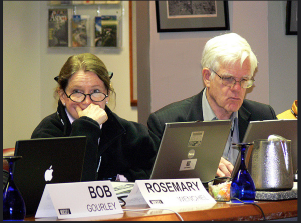
\includegraphics{1.1.png}
\caption{\emph{Linton Wells II (derecha), ex director de información y
adjunto de defensa para las redes, en una reciente sesión del Foro
Highlands del Pentágono. Rosemary Wenchel, un alto funcionario del
Departamento de Seguridad Nacional, está sentada a su lado}}
\end{figure}

La revista \emph{New Scientific} (de acceso web mediante pago) ha
comparado al Foro Highlands con reuniones de élite tales como ``Davos,
Ditchley y Aspen'', describiéndola como ``mucho menos conocida,
pero\ldots{} sin duda tan influyente como las reuniones de negocios''.
Las reuniones periódicas del Foro juntan a ``personas innovadoras para
considerar las interacciones entre la política y la tecnología. Sus
mayores éxitos han sido en el desarrollo de la guerra de alta tecnología
basada en la red''.

Dado el papel de Wells en ese foro, tal vez no fue sorprendente que su
libro blanco para la transformación de la defensa fuera capaz de tener
un profundo impacto sobre la actual política del Pentágono. Pero si ese
fuera el caso, ¿por qué nadie lo notó?

A pesar de estar patrocinado por el Pentágono, no se podía encontrar
ninguna página oficial en el sitio web del DoD sobre el Foro. Fuentes de
inteligencia y militares de EE.UU. activas y retiradas nunca habían oído
hablar de él, y tampoco los periodistas de seguridad nacional. Me sentí
frustrado.

\subsection{La empresa de riesgo de capital intelectual del
Pentágono}\label{la-empresa-de-riesgo-de-capital-intelectual-del-pentuxe1gono}

En el prólogo de su libro de 2007, \emph{Una multitud de uno: el futuro
de la identidad individual}, John Clippinger, un científico del MIT del
Grupo de Dinámicas Humanas del Laboratorio de Medios, describió su
participación en una reunión del ``Foro Highlands'', una ``reunión sólo
para invitados financiada por el Departamento de Defensa y presidida por
el asistente para la integración de redes e información''. Este era un
cargo de alto rango del DoD que supervisaba operaciones y políticas para
las más poderosas agencias de espionaje del Pentágono incluyendo la NSA
y la Agencia de Inteligencia de Defensa (DIA), entre otras. A partir de
2003, la posición fue una transición hacia lo que ahora es el
subsecretario de defensa para inteligencia. El Foro Highlands, escribió
Clippinger, fue fundado por un capitán retirado de la Marina de EE.UU.
llamdo Dick O'Neill. Los delegados incluyen oficiales militares de alto
rango de EE.UU. pertenecientes a numerosas agencias y divisiones -
``capitanes, contraalmirantes, generales, coroneles, mayores y
comandantes'' así como ``miembros líderes del DoD.''

Lo que al principio parecía ser el principal sitio web del Foro describe
a Highlands como ``una red informal interdisciplinaria patrocinada por
el Gobierno Federal'', enfocada en la ``información, la ciencia y la
tecnología''. La explicación es escasa, más allá del simple logo del
``Departamento de Defensa''.

Pero Highlands tiene también otro sitio web que se describe a sí mismo
como una ``empresa de riesgo de capital intelectual'' con ``extensa
experiencia asistiendo a corporaciones, organizaciones y líderes del
gobierno''. La empresa provee un ``amplio rango de servicios,
incluyendo: planeamiento estratégico, creación de escenarios y juegos
para la expansión de mercados globales'', así como ``trabajo con
clientes para construir estrategias para la ejecución''. El Grupo
Highlands Inc., dice el sitio web, organiza un completo rango de foros
sobre el tema.

Por ejemplo, además del Foro Highlands, desde el 11-S el Grupo organiza
el ``Foro Island'', un evento internacional mantenido en asociación con
el Ministro de Defensa de Singapur, el cual O'Neill supervisa como
``líder consultor''. El sitio web del Ministerio de Defensa de Singapur
describe al Foro Island como ``modelado después del Foro Highlands
organizado por el Departamento de Defensa de los EE.UU.'' Los documentos
revelados por el informante Edward Snowden confirman que Singapur jugó
un papel clave al ṕermitir que los EE.UU. y Australia interceptaran
cables submarinos para espiar a potencias asiáticas como Indonesia y
Malasia..

El sitio web del Grupo Highlands también revela que Highlands es un
socio de uno de los mayores contratistas de defensa de los EE.UU.
Highlands está ``apoyado por una red de compañías e investigadores
independientes'', que incluyen a ``nuestros socios del Foro Highlands
por los últimos diez años en SAIC; y la amplia red de participantes en
el Foro Highlands''.

SAIC es la sigla de la empresa de defensa de los EE.UU, Science
Applications International Corporation (Corporación Internacional de
Aplicaciones de la Ciencia), que cambió su nombre a Leidos en el 2013,
que opera a SAIC como una subsidiaria. SAIC/Leidos está entre los diez
contratistas de defensa más grandes, y trabaja estrechamente con la
comunidad de inteligencia de los EE.UU., especialmente la NSA. Según el
periodista de investigación Tim Shorrock, el primero en revelar la
amplia extensión de la privatización de la inteligencia en EE.UU. con su
trascendental libro \emph{Spies for Hire}, SAIC tiene una ``relación
simbiótica con la NSA: la agencia es el mayor cliente individual de la
compañía y SAIC es el mayor contratista de la NSA''.

\begin{figure}[htbp]
\centering
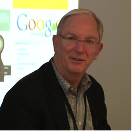
\includegraphics{1.2.png}
\caption{\emph{Richard `Dick' Patrick O'Neill, fundador y presidente del
Foro Highlands del Pentágono}}
\end{figure}

El nombre completo del capitán ``Dick'' O'Neill, el presidente fundador
de Foro Highlands, es Richard Patrick O'Neill, quien después de su
trabajo en la Marina se unió al DoD. Desempeñó su último cargo como
asistente para la estrategia y la política en la Oficina del Secretario
Adjunto de Defensa para el Comando, Control, Comunicaciones e
Inteligencia, antes de la fundación de Highlands.

\subsection{El Club de Yoda}\label{el-club-de-yoda}

Pero Clippinger también se refiere a otro individuo misterioso venerado
por los concurrentes al Foro:

\begin{quote}
\emph{``Se sentó en la parte de atrás de la sala, sin ninguna expresión
detrás de sus gruesos anteojos, de montura negra. Nunca le escuché
pronunciar una palabra\ldots{} Andrew (Andy) Marshall es un ícono dentro
del DoD. Algunos lo llaman Yoda, por su mítico estado de
inescrutabilidad\ldots{} Él se ha desempeñado en varias administraciones
y ha tenido una amplia consideración por sobre la política partidista.
Fue un partidario del Foro Highlands y un asistente regular desde su
comienzo''.}
\end{quote}

Desde 1973 Marshall encabezaba una de las más poderosas agencias del
Pentágono, la Oficina de Evaluación de Red (ONA), el think tank interno
del secretario de defensa de los EE.UU. que conduce la investigación
altamente clasificada sobre el planeamiento futuro de la política de
defensa a través de la comunidad de inteligencia y militar de los EE.UU.
La ONA ha desempeñado un rol clave en las principales iniciativas
estratégicas del Pentágono, incluyendo la Estrategia Marítima, la
Iniciativa para la Defensa Estratégica, la Iniciativa de Estrategias
Competitivas y la Revolución en Asuntos Militares.

\begin{figure}[htbp]
\centering
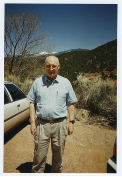
\includegraphics{1.3.png}
\caption{\emph{Andrew `Yoda' Marshall, director de la Oficina de
Evaluación de la Red (ONA) y codirector del Foro Highlands, en un
antiguo evento del Foro Highlands en 1996 en el Instituto Santa Fe.
Marshall se retiró en enero del 2015}}
\end{figure}

En una extraña semblanza en 2002 en \emph{Wired}, el reportero Douglas
McGray describió a Andrew Marshall, actualmente de 93 años de edad, como
``el más esquivo del DoD'' pero ``uno de los más influyentes''
funcionarios. McGray añadió que ``el vicepresidente Dick Cheney, el
secretario de defensa Donald Rumsfeld, y el subsecretario Paul
Wolfowitz'' - ampliamente considerados los halcones del movimiento
neoconservador en la política norteamericana - fueron algunas de los
``estrellas protegidas'' de Marshall.

Hablando en un sencillo seminario en la Universidad de Harvard después
del 11-S, el presidente fundador del Foro Highlands Richard O'Neill dijo
que Marshall fue mucho más que un ``asistente regular'' al Foro. ``Andy
Marshall es nuestro co-presidente, por lo que indirectamente todo lo que
hacemos se remonta al sistema de Andy'', le dijo a la audiencia.
``Directamente, las personas que asisten a las reuniones del Foro pueden
pasar sus informes a Andy sobre una variedad de tópicos y sintetizar
cosas''. También dijo que el Foro tiene un tercer co-presidente: el
director de la Agencia de Proyectos e Investigación en Defensa Avanzada
(DARPA), que al mismo tiempo era un elegido de Rumsfeld, Anthony J.
Theter. Antes de unirse a DARPA, Tether era vicepresidente del Sector de
Tecnología Avanzada de SAIC.

\begin{figure}[htbp]
\centering
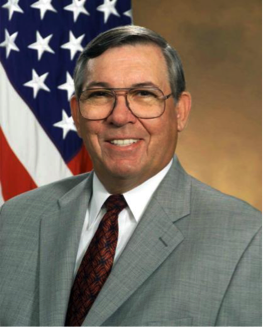
\includegraphics{1.4.png}
\caption{\emph{Anthony J. Tether, director de DARPA y codirectordel Foro
Highlands del Pentágono desde junio de 2001 a febrero de 2009}}
\end{figure}

La influencia del Foro Highlands sobre la política de defensa de EE.UU.
ha operado de este modo a través de tres canales principales: el
patrocinio de la oficina del Secretario de Defensa (alrededor de la
mitad de la década pasada fue transferida específicamente a la oficina
del Subsecretario de Defensa para Inteligencia, que está a cargo de las
principales agencias de vigilancia), conectada directamente con la ONA
de Andrew Marshall; esta última vinculada con DARPA.

\begin{figure}[htbp]
\centering
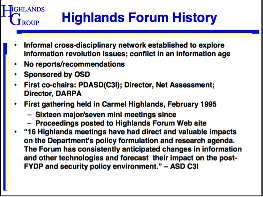
\includegraphics{1.5.png}
\caption{\emph{Una diapositiva de la presentación de Richard O'Neill en
la Universidad de Harvard en 2001}}
\end{figure}

De acuerdo a Clippinger en \emph{Una multitud de uno}, ``lo que sucede
en reuniones informales tales como en el Foro Highlands, tiene un enorme
impacto con el tiempo, a través de curiosas e inesperadas vías de
influencia, no sólo dentro del DoD sino también en todo el mundo''. El
escribió que las ideas del Foro han ``pasado de ser herejías a ser
convencionales. Ideas que eran anatemas en 1999 han sido adoptadas como
políticas sólo tres años más tarde''.

Aunque el Foro no produce ``recomendaciones consensuadas'', su impacto
es más profundo que el de un tradicional comité asesor del gobierno.
``Las ideas que surgen de las reuniones están disponibles para su uso
por parte de los tomadores de decisiones así como para la gente de los
thinks tanks,'' de acuerdo a O'Neill:

\begin{quote}
\emph{Vamos a incluir personas de Booz, SAIC, RAND, u otras de nuestras
reuniones\ldots{} Damos la bienvenida a ese tipo de cooperación, porque,
verdaderamente, ellos son importantes. Están allí a largo plazo y son
capaces de influir en las políticas gubernamentales con trabajo muy
académico\ldots{} Nosotros producimos ideas e interacción y redes para
que estas personas las puedan tomar y usar cuando lo necesiten.}
\end{quote}

Mis repetidas requisitorias a O'Neill para saber de su trabajo en Foro
Highlands fueron ignoradas. El Departamento de Defensa tampoco respondió
a mis múltiples pedidos de información ni hizo comentarios acerca del
Foro.

\subsection{La guerra de la
información}\label{la-guerra-de-la-informaciuxf3n}

El Foro Highlands ha servido como un ``puente para el tráfico de
influencias'' en dos sentidos: en un sentido, para la influencia de la
red oculta de contratistas privados en la formulación de operaciones de
información a través de la inteligencia militar de los EE.UU., y en el
otro, para la influencia del Pentágono sobre el sector privado. No hay
evidencia más clara de esto que el papel verdaderamente instrumental del
Foro en la incubación de la idea de la vigilancia global como mecanismo
para dominar la información a escala mundial.

En 1989, Richard O'Neill, entonces un criptógrafo de la Marina
estadounidense, escribió un paper para el Colegio de Guerra Naval de
EE.UU., \emph{Hacia una metodología para el manejo de las percepciones}.
En su libro, \emph{Future Wars}, el Coronel John Alexander, entonces un
oficial superior del Comando de Seguridad e Inteligencia de la Marina de
los EE.UU. (INSCOM), mencionó que el paper de O'Neill delineó por
primera vez una estrategia para el ``manejo de las percepciones'' como
parte de la guerra de información (IW). Las estrategias propuestas por
O'Neill identificaron tres categorías de objetivos para la IW:
adversarios, para que se sientan vulnerables; socios potenciales, ``para
que perciben la causa (de la guerra) como justa''; y, finalmente, la
población civil y los líderes políticos para que ``perciban el costo
como un mérito al esfuerzo''. Una informe secreto basado en el trabajo
de O'Neill ``llegó a la cúpula'' del DoD. ``Reconocieron que O'Neill
tenía razón y le dijeron que lo archivara''.

Excepto que el DoD no lo archivó. Alrededor de 1994, el Grupo Highlands
fue fundado por O'Neill como un proyecto oficial del Pentágono por el
nombramiento del entonces secretario de defensa de Bill Clinton, William
Perry - quien se unió a la junta directiva de SAIC después de retirarse
del gobierno en 2003.

En las propias palabras de O'Neill, el grupo funcionaría como un
``laboratorio de ideas'' del Pentágono. Según \emph{Government
Executive}, expertos en tecnología de la información (IT) y militares
asistieron a la primera reunión del Foro ``para considerar el impacto de
la IT y la globalización en los EE.UU. y en la guerra. ¿Cómo podrían
cambiar al mundo Internet y otras tecnologías emergentes?''. La reunión
ayudó a sembrar la idea de la ``guerra centrada en las redes'' en la
mente de los ``pensadores militares más influyentes de la nación''.

\subsection{Excluyendo al público}\label{excluyendo-al-puxfablico}

Los registros oficiales del Pentágono confirman que el objetivo primario
fue apoyar a la políticas del DoD en la especialidad de O'Neill: la
guerra de la información. Según el Reporte Anual del Pentágono de 1997
para el Presidente y el Congreso bajo una sección titulada ``Operaciones
de información'' (IO), la Oficina de la Secretaría de Defensa (OSD) ha
autorizado la ``creación del Grupo Highlands en el contexto del DoD, la
industria y los expertos académicos en IO'' para coordinar las IO a
través de las agencias federales de inteligencia militar.

Los años siguientes el reporte anual del DoD reiteraba el enfoque del
Foro en las operaciones de información: ``Para examinar los temas de IO,
el DoD patrocina el Foro Highlands, el cual trabaja junto al gobierno,
la industria y los profesionales académicos de diferentes campos.''

Vale resaltar que en 1998, el ``Grupo'' Highlands se convirtió en
``Foro''. Según O'Neill, esto se hizo para evitar que las reuniones del
Foro Highlands quedaran sujetas a ``restricciones burocráticas''. A lo
que él estaba haciendo alusión era la Ley Federal de Comité Consultivo
(FACA), que regula la forma en que el gobierno estadounidense puede
solicitar formalmente el asesoramiento de intereses especiales.

Conocida como la ley de ``gobierno abierto'', FACA requiere que los
oficiales de gobierno de EE.UU. no puedan manejarse a puertas cerradas
ni mantener consultas secretas con personas externas al gobierno para
desarrollar políticas. Todas estas consultas deberían tener lugar por
medio de los comités de asesoramiento federales que permiten el control
público. FACA requiere que las reuniones sean públicas, anunciadas por
intermedio del Registro Federal, que los grupos de asesores estén
registrados en la Administración de Servicios Generales, además de otros
requerimientos pensados para mantener la rendición de cuentas ante el
interés público.

Pero \emph{Government Executive} reportó que ``O'Neill y otros creían''
que tales cuestiones reglamentarias ``podrían entorpecer el libre flujo
de ideas y las discusiones sin tapujos que buscaban''. Los abogados del
Pentágono advirtieron que la palabra ``Grupo'' podría acarrear ciertas
obligaciones y sugirieron dejar todo en manos privadas: ``Entonces
O'Neill cambió el nombre a Foro Highlands y lo trasladó al sector
privado para manejarlo como consultor del Pentágono''. El Foro Highlands
del Pentágono entonces funciona bajo el manto de la ``empresa de riesgo
de capital intelectual'' de O'Neill, ``Highlands Group Inc.''.

En 1995, un año después que William Perry designara a O'Neill a la
cabeza del Foro Highlands, SAIC - la organización ``socia'' del Foro -
inauguró un nuevo Centro para la Política y Estrategia de la Información
bajo la dirección de ``Jeffrey Cooper, un miembro del Grupo Highlands
que asesoraba a oficiales superiores del Departamento de Defensa en
cuestiones referidas a la guerra de la información''. El Centro tuvo
precisamente el mismo objetivo que el Foro, funcionar como ``un centro
de consulta para reunir a las mejores y más brillantes mentes en guerra
de la información con el patrocinio de una serie de seminarios,
ponencias y simposios que exploren las implicancias de la guerra de la
información en profundidad''. El objetivo era ``permitir que los
dirigentes y autoridades gubernamentales, industriales y académicas
pudieran abordar las cuestiones claves alrededor de la guerra de la
información para asegurar que Estados Unidos conserve su ventaja sobre
todos sus enemigos potenciales''.

A pesar de las regulaciones de la FACA, los comités asesores federales
están muy fuertemente influenciados, cuando no manejados, por el poder
corporativo. Así que al eludir la FACA, el Pentágono omitió incluso sus
restricciones menores, al excluir permanentemente toda posibilidad de
participación del público.

La afirmación de O'Neill de que no existen informes o recomendaciones es
falsa. Por reconocimiento propio, las consultas secretas del Pentágono
con la industria que han tenido lugar a través del Foro Highlands desde
1994 han sido acompañadas por las presentaciones regulares de papers
políticos y académicos, grabaciones y notas de reuniones y otras formas
de documentación que están bajo llave y son sólo accesibles para los
delegados del Foro. Esto viola el espíritu, si no la letra, de la FACA
--- en una forma donde claramente se pretende eludir la responsabilidad
democrática y el estado de derecho.

El Foro Highlands no necesita producir recomendaciones consensuadas. Su
propósito es proveerle al Pentágono un mecanismo oculto en las redes
sociales para consensuar relaciones duraderas con el poder corporativo,
e identificar nuevos talentos, que pueden usarse para ajustar las
estrategias en la guerra de la información en un absoluto secreto.

El número total de participantes en el Foro Highlands del DoD supera los
mil, aunque las sesiones consisten en gran parte de reuniones al estilo
de pequeños talleres cerrados de 25 a 30 personas como máximo, que
reúnen a expertos y funcionarios dependiendo del tema. Los delegados han
incluído a personal de alto rango de SAIC y Booz Allen Hamilton, RAND
Corp., Cisco, Human Genome Sciences, eBay, PayPal, IBM, Google,
Microsoft, AT\&T, la BBC, Disney, General Electric, Enron, entre muchos
más; miembros del Congreso y el Senado demócratas y republicanos; altos
ejecutivos de la industria de la energía de EE.UU. como Daniel Yergin de
IHS Cambridge Energy Research Associates; y personal clave involucrado
en ambos lados de las campañas presidenciales.

Otros participantes son profesionales de alto nivel de los medios de
comunicación: David Ignatius, editor asociado del Washington Post y al
tiempo editor ejecutivo del International Herald Tribune; Thomas
Friedman, columnista del New York Times desde hace mucho tiempo; Arnaud
de Borchgrave, editor en el Washington Times y en United Press
International; Steven Levy, un ex editor de Newsweek, escritor senior
para Wired y ahora editor en jefe de tecnología en Medios; Lawrence
Wright, redactor en el New Yorker; Noah Shachtmann, editor ejecutivo en
el Daily Beast; Rebecca McKinnon, cofundadora de Global Voices Online;
Nik Gowing de la BBC; y John Markoff del New York Times.

Debido al patrocinio actual del subsecretario de defensa para
inteligencia del OSD, el Foro tiene acceso interno a los jefes de las
principales agencias de reconocimiento y vigilancia de los EE.UU., así
como a los directores y sus asistentes en las agencias de investigación
del DoD, desde DARPA hasta ONA. Esto también significa que el Foro está
profundamente conectado con los equipos de tareas de investigación
política del Pentágono.

\subsection{Google: sembrado por el
Pentágono}\label{google-sembrado-por-el-pentuxe1gono}

En 1994 - el mismo año en que el Foro Highlands fue fundado bajo la
tutela de la oficina del secretario de defensa, la ONA, y DARPA - dos
jóvenes estudiantes de doctorado de la Universidad de Stanford, Sergey
Brin y Larry Page, obtuvieron un logro con su primera aplicación de
ranking de páginas web e indexado automatizado. Esta aplicación
permanece como un componente central de lo que con el tiempo se
convirtió en el servicio de búsqueda de Google. Brin y Page han
realizado su trabajo con el financiamiento de la Iniciativa de
Bibliotecas Digitales (DLI), un programa de múltiples agencias de la
Fundación Nacional de Ciencias (NSF), la NASA y DARPA.

Pero esto es sólo una parte de la historia.

Durante el desarrollo del motor de búsqueda, Sergey Brin reportaba
regular y directamente a dos personas que no pertenecían en absoluto a
la facultad de Stanford: la Dra. Bhavani Thuraisingham y el Dr.~Rick
Steinheiser. Ambos eran representantes de sensibles programas de
investigación de la comunidad de inteligencia de los EE.UU. sobre
seguridad de la información y data mining.

Thuraisingham es actualmente el profesor distinguido Louis A. Beecherl y
el director ejecutivo del Instituto de Investigaciones sobre
Ciberseguridad de la Universidad de Texas, Dallas, y una experta
cotizada en data mining, administración de datos y en temas de seguridad
de la información. Pero en los '90, ella trabajaba para MITRE Corp., un
contratista líder de defensa de EE.UU. donde administraba la iniciativa
de sistemas de datos digitales masivos, un proyecto patrocinado por la
NSA, la CIA y el Director de la Central de Inteligencia, para promover
investigaciones innovadoras en tecnología de la información.

``Hemos financiado a la Universidad de Stanford a través del experto en
informática Jeffrey Ullman, quien tenía varios estudiantes graduados
promisorios trabajando en muchas áreas excitantes,'' me dijo la prof.
Thuraisingham. ``Uno de ellos era Sergey Brin, el fundador de Google. El
programa MDDS de la comunidad de inteligencia en esencia le proporcionó
un capital inicial de inversión a Brin, que fue complementada por muchas
otras fuentes, incluyendo el sector privado''.

Esta forma de financiamiento ciertamente no es inusual, y que Sergey
Brin fuera autorizado para recibirla siendo un estudiante graduado
parece haber sido casual. El Pentágono había terminado sus
investigaciones sobre la ciencia de la computación en ese tiempo. Pero
esto ilustra cuán profundamente estaba arraigada la cultura de Silicon
Valley en los valores de la comunidad de inteligencia de los EE.UU.

En un extraordinario documento hospedado en el sitio web de la
Universidad de Texas, Thuraisingham relata que desde 1993 a 1999, ``la
Comunidad de Inteligencia (IC) comenzó un programa denominado Sistemas
de Datos Digitales Masivos (MDDS) que administré para la Comunidad de
Inteligencia cuando estaba en MITRE Corporation''. El programa financió
15 esfuerzos de investigación de varias universidades, incluyendo
Stanford. Su meta era desarrollar ``tecnologías de administración de
datos para manejar desde varios terabytes a petabytes de datos,''
incluso para ``procesamiento de consultas, manejo de transacciones,
manejo de metadatos, administración de almacenamiento e integración de
datos''.

En ese momento, Thuraisingham era científica en jefe para el manejo de
información y datos de MITRE, donde lideraba los esfuerzos del equipo de
investigación y desarrollo para la NSA, la CIA. el Laboratorio de
Investigación de la Fuerza Aérea, así como también el Comando de
Sistemas de Guerra Espacial y Naval de la Marina de los EE.UU.(SPAWAR) y
el Comando Electrónico y de Comunicaciones (CECOM). Ella impartía cursos
para funcionarios de gobierno de los EE.UU. y contratistas de defensa
sobre datamining en contraterrorismo.

En su artículo de la Universidad de Texas, ella adjuntó la copia de una
reseña sobre el programa MDDS de la comunidad de inteligencia de los
EE.UU. que había sido presentada en el ``Simposio Anual de la Comunidad
de Inteligencia'' en 1995. La reseña revela que los patrocinantes
principales del programa MDDS fueron tres agencias: la NSA, la Oficina
de Investigación y Desarrollo de la CIA y el Grupo de Gestión de la
Comunidad (CMS) de inteligencia que opera bajo órdenes del Director de
la Central de Inteligencia. Los administradores del programa, que
aportaron 3 o 4 millones de dólares de financiamiento por año durante 3
o 4 años, fueron identificados como Hal Curran (NSA), Robert Kluttz
(CMS), Dra. Claudia Pierce (NSA), Dr.~Rick Steinheiser (ORD, la oficina
de investigación y desarrollo de la CIA) y la Dra. Thuraisingham en
persona.

Thuraisingham vuelve a reiterar en su artículo que este programa
conjunto entre la CIA y la NSA financió parcialmente a Sergey Brin para
desarrollar el núcleo central de Google, a través de una subvención a
Stanford manejada por el supervisor de Brin, el profesor Jeffrey
D.Ullman:

\begin{quote}
\emph{De hecho, el fundador de Google el Sr. Sergey Brin fue
parcialmente financiado por este programa mientras era un estudiante de
doctorado en Stanford. Junto con su tutor Prof.~Jeffrey Ullman y mi
colega en MITRE Dr.~Chris Clifton (jefe científico en TI de MITRE),
desarrolló el sistema Quey Flocks que arrojaba soluciones para la
extracción de enormes cantidades de datos almacenadas en las bases de
datos. Recuerdo visitar Stanford con el Dr.~Rick Stenheiser de la
comunidad de inteligencia y el Sr. Brin solía irrumpir en patines, dar
su presentación y retirarse velozmente. De hecho la última vez que nos
reunimos en septiembre de 1998, el Sr. Brin nos demostró su motor de
búsqueda que se convertiría en Google poco después.}
\end{quote}

Brin y Page constituyeron oficialmente a Google como una empresa en
septiembre de 1998, el mismo mes que reportaron por última vez a
Thuraisingham y Steinheiser. ``Query flocks'' también forma parte del
sistema de búsqueda patentado de Google, ``PageRank'', que Brin
desarrolló en Stanford bajo el programa de la CIA, la NSA y MDDS, así
como también con financiamiento de NSF, IBM e Hitachi. Ese año, el
Dr.~Chris Clifton de MITRE, que trabajó bajo las órdenes de
Thuraisingham para desarrollar el sistema ``Query flocks'', escribió un
paper en coautoría con el supervisor de Brin, el Prof.Ullman, y el de la
CIA Rick Steinheiser. Titulado \emph{Descubriendo información en
textos}, el paper fue presentado en una conferencia académica.

``El financiamiento de MDDS que patrocinó a Brin fue significativo en
cuanto a los fondos iniciales, pero probablemente fue superado por otras
fuentes de financiación'', dijo Thuraisingham. ``La duración del
financiamiento a Brin fue de alrededor de dos años aproximadamente. En
ese período, junto a mis colegas del MDDS visitábamos Stanford para ver
a Brin y monitorear su progreso cada tres meses aproximadamente. No
éramos exactamente sus supervisores, pero queríamos comprobar su
progreso, señalar los potenciales problemas y sugerir ideas. En aquellas
sesiones informativas, Brin nos presentó su investigación sobre query
flocks, y también nos demostró las versiones preliminares del motor de
búsqueda de Google''.

Hasta aquí, Brin reportó a Thuraisinghaim y a Steinheiser regularmente
acerca de su trabajo desarrollando Google. El programa MDDS es
mencionado actualmente en varios papers con la coautoría de Brin y Page
mientras asistían a Stanford. En su paper publicado en 1998 en el
Boletín del Comité Técnico Social de Computación sobre Ingeniería de
Datos de la IEEE, describen la automatización de los métodos de
extracción de información a partir de la web por medio de la
``extracción por patrones de relación iterativos duales'', el desarrollo
de un ``ranking global de páginas web denominado PageRank'', y el uso de
PageRank para ``desarrollar un nuevo motor de búsqueda llamado Google''.
En una nota al pie de página en la apertura, Sergey Brin confirma que él
estaba ``parcialmente patrocinado por el Programa de Sistemas Digitales
Masivos de Datos del Equipo Administración de la Comunidad'', a través
de una subvención de la NSF - confirmando que el programa de la CIA, la
NSA y el MDDS aportó sus financiamiento a través de la NSF.

Esta subvención , cuyo informe del proyecto menciona a Brin entre los
estudiantes beneficiarios (sin mencionar al MDDS), era diferente a la
subvención a Larry Page que incluyó financiamiento de DARPA y la NASA.
El reporte del proyecto. autorizado por el supervisor de Brin,
Prof.Ullman, continúa diciendo bajo la sección ``Indicaciones de éxito''
que ``hay algunas nuevas historias de nuevas empresas basadas en la
investigación apoyada por la NSF''. Bajo ``Impacto del proyecto'', el
reporte señala: ``Finalmente, el proyecto google también se ha vuelto
comercial con Google.com''.

La explicación de Thuraisingham por lo tanto demuestra que el programa
de la CIA, la NSA y MDDS no sólo financió a Brin a través de su trabajo
con Larry Page desarrollando Google, sino también que los representantes
de alto nivel de la inteligencia de los EE.UU. incluyeron a un oficial
de la CIA que supervisó la evolución de Google en su fase de
pre-lanzamiento, durante todo el camino hasta que la empresa estuvo
lista para ser oficialmente fundada. Google, entonces, fue activada con
una ``significativa'' cantidad de capital inicial y supervisada desde el
Pentágono: a saber, la CIA, la NSA y DARPA.

El DoD no hizo comentarios al respecto.

Cuando le pregunté al Prof.~Ullman para confirmar si Brin fue
parcialmente financiado o no por el programa MDDS de la comunidad de
inteligencia, y si Ullman era consciente de que Brin era supervisado
regularmente por Rick Steinheiser de la CIA mientra desarrollaba el
motor de búsqueda Google, Ullman respondió de forma evasiva: ``¿Puedo
saber a quién representa usted y por qué está interesado en estas
cuestiones?¿Quiénes son sus''fuentes``? También negó que Brin haya
desempeñado un rol importante en el desarrollo del sistema de''query
flocks``, aunque queda claro a partir de los papers de Brin que se
inspiró en este trabajo para desarrollar junto a Page el sistema
PageRank.

Cuando le pregunté a Ullman si el estaba negando el rol de la comunidad
de inteligencia de los EE.UU. apoyando a Brin durante el desarrollo de
Google, respondió: ``No me voy a dignar a responder esta tontería con
una negación. Si no me explica cuál es su teoría, y qué es lo que está
tratando de hacer, no voy a ayudarlo en lo más mínimo''.

La reseña del MDDS publicada online por la Universidad de Texas confirma
que la razón de ser del proyecto de la CIA y la NSA era ``proveer un
capital inicial para desarrollar tecnologías de administración de datos
de alto riesgo y altos dividendos'', incluyendo técnicas para
``consultas, navegación y filtrado, procesamiento de transacciones,
métodos de acceso e indexación, gestión de metadatos y modelado de
datos, e integración de bases de datos heterogéneas, así como el
desarrollo de arquitecturas apropiadas''. La visión de máxima del
programa era ``procurar el acceso constante y la fusión de cantidades
enormes de datos, información y conocimientos en un medio ambiente
heterogéneo en tiempo real'' para ser usado por el Pentágono, la
comunidad de inteligencia y potencialmente el gobierno.

Estas revelaciones corroboran la declaración de Robert Steele, ex
oficial de alto rango de la CIA y subdirector civil fundador de la
Actividad de Inteligencia del Cuerpo de Marines, a quien entrevisté para
el periódico \emph{The Guardian} el año pasado en referencia a la
inteligencia open source. Citando fuentas de la CIA, Steele dijo que en
2006 Steinheiser, un viejo colega suyo, fue el enlace de la CIA en
Google que proporcionó los primeros fondos para la firma de IT pionera.
Al mismo tiempo, el fundador de \emph{Wired} John Batelle logró obtener
esta negación oficial de un portavoz de Google en respuesta a las
afirmaciones de Steele:

\begin{quote}
\emph{``Las declaraciones relacionadas a Google son completamente
falsas''.}
\end{quote}

En esta ocasión, a pesar de múltiples pedidos y conversaciones, un
vocero de Google rechazó hacer declaraciones.

ACTUALIZACIÓN: a las 5:41PM GMT, el Director de comunicación corporativa
de Google se puso en contacto conmigo y me pidió que incluyera la
siguiente declaración:

\begin{quote}
\emph{``Sergey Brin no formaba parte del Programa Query Flocks en
Stanford, y ninguno de sus proyectos fueron financiados por los
organismos de inteligencia de EE.UU''.}
\end{quote}

Mi contestación es la siguiente:

Mi respuesta a esta declaración es la siguiente: el propio Brin en su
paper reconoce el financiamiento de la iniciativa MDDS (Sistemas de
Datos Digitales Masivos) del CMS (Equipo de Administración de la
Comunidad) que fue suministrada a través de lla NSF. MDDS fue un
programa de la comunidad de inteligencia generado por la CIA y la NSA.
También me consta , como se observa en una parte, que la
Prof.~Thurainsingham de la Universidad de Texas administraba el programa
MDDS en representación de la comunidad de inteligencia de EE.UU., y que
ella y Rick Steinheiser de la CIA se reunieron con Brin cada tres meses
aproximadamente durante dos años para supervisar el progreso del
desarrollo de Google y PageRank. Si Brin trabajó en query flocks no se
sabe con exactitud.

En este contexto, usted se podría preguntar lo siguiente:

\begin{enumerate}
\def\labelenumi{\arabic{enumi})}
\item
  ¿Google niega que el trabajo de Brin fue parcialmente financiado por
  el MDDS por medio de una subvención de la NSF?
\item
  ¿Google niega que Brin reportaba regularmente a Thurainsingham y
  Steinheiser desde alrededor de 1996 hasta septiembre de 1998, el año
  en que les fue presentado a ellos el motor de búsqueda Google?
\end{enumerate}

\subsection{Conocimiento total de la
información}\label{conocimiento-total-de-la-informaciuxf3n}

El 3 de noviembre de 1993 se publicó la apertura del plazo de recepción
de papers para el MDDS por medio de una lista de correos electrónicos
del oficial de alto rango de la inteligencia de EE.UU. David Charvonia,
director de la oficina de coordinación de investigación y desarrollo del
CMS de la comunidad de inteligencia. La reacción de Tatu Ylonen (famoso
inventor del ampliamente usado protocolo de protección de datos de shell
segura (SSH)) fue decirles a sus colegas en la lista de correos
electrónicos: ``¿Cripto relevancia? Te hace pensar si debes proteger tus
datos''. El mensaje también confirma que el contratista de defensa y
socio del Foro Highlands, SAIC, manejó el proceso de presentaciones a
MDDS con reseñas que fueron enviadas a Jackie Booth de la Oficina de
Investigación y Desarrollo de la CIA por intermedio de una dirección de
correo electrónico de SAIC.

En 1997, revela Thuraisingham, poco antes que Google fuera lanzada como
empresa y mientras ella aún supervisaba el desarrollo de este motor de
búsqueda en Stanford, enfocó sus pensamientos en las aplicaciones de
seguridad nacional del programa MDDS. En los agradecimientos de su libro
\emph{Web Data Mining y aplicaciones en inteligencia de negocios y
contraterrorismo} del año 2003, Thuraisingham escribió que ella y el
``DR.Rick Steinheiser de la CIA, comenzaron a discutir con la Agencia de
Proyectos de Investigación Avanzada en Defensa acerca de las
aplicaciones del data mining en contraterrorismo'', una idea que se
originó directamente desde el programa MDDS que financió parcialmente a
Google. ``Estas discusiones con el tiempo se convirtieron en el actual
programa de DARPA, EELD (Detección de Enlaces y Extracción de
Evidencias)''

Entonces el mismo oficial superior de la CIA y contratista de la CIA y
la NSA involucrado en el suministro del capital inicial para Google
estaba considerando simultáneamente el rol del data mining para
propósitos contraterroristas, y estaba desarrollando ideas para
herramientas de hecho expuestas por DARPA.

Hoy, como lo demuestra su reciente página de opinión en \emph{The New
York Times}, Thuraisingham continúa siendo una defensora acérrima del
data mining con propósitos contraterroristas, pero también insiste que
estos métodos deben ser desarrollados por el gobierno en cooperación con
los abogados de libertades civiles y defensores privados para asegurar
que estos procedimientos robustos se apliquen para impedir potenciales
abusos. Ella señala, críticamente, que con la cantidad de información
que está siendo recolectada, existe un alto riesgo de falsos positivos.

En 1993, cuando el programa MDDS fue lanzado y administrado por MITRE
Corp. en representación de la comunidad de inteligencia de EE.UU., la
experta en informática de la Universidad de Virginia, Dra. Anita K.
Jones - miembro del consejo de administración de MITRE - obtuvo el
puesto de director de DARPA y jefe de investigación e ingeniería a
través del Pentágono. Ella ha estado en la junta de MITRE desde 1988.
Entre 1987 y 1993, Jonas simultáneamente sirvió en la junta directiva de
SAIC. Como nuevo jefe de DARPA desde 1993 a 1997, ella también codirigió
el Foro Highlands del Pentágono durante el período de desarrollo y
prelanzamiento de Google en Stanford a cargo del MDSS.

Así, cuando Thuraisingham y Steinheiser hablaban en DARPA sobre las
aplicaciones del contraterrorismo de la investigación del MDDS, Jones
era director de DARPA y Co-Presidente del Foro Highlands. Ese mismo año,
Jones dejó DARPA para volver a su puesto en la Universidad de Virgina.
Al año siguiente, se incorporó a la Junta de la Fundación Nacional de
Ciencia (NSF) de EE.UU., que por supuesto había financiado también a
Brin y Page y también volvió a la Junta Directiva de SAIC. Cuando dejó
el DoD, el senador Chuck Robb le brindó a Jones el siguiente tributo:
``Trajo la tecnología y las comunidades militares operativas unidas para
diseñar planes detallados para mantener el dominio de Estados Unidos en
el campo de batalla en el próximo siglo''.

\begin{figure}[htbp]
\centering
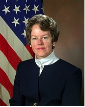
\includegraphics{1.6.png}
\caption{\emph{Dra. Anita Jones, jefa de DARPA de 1993 a 1997, y
codirectora del Foro Highlands del Pentágono de 1995 a 1997; en ese
lapso de tiempo funcionarios a cargo del programa de la CIA-NSA-MDSS
financiaron Google, y estuvieron en contacto con DARPA en relación a la
minería de datos para el contraterrorismo}}
\end{figure}

En la junta de la Fundación Nacional de Ciencia desde 1992 a 1998
(incluyendo un período como jefe desde 1996) estaba Richard N. Zare.
Este fue el período en que la NSF patrocinó a Sergey Brin y Larry Page
en asociación con DARPA. En junio de 1994, el Prof.~Zare, un químico de
Stanford, participó con el Prof.~Jeffrey Ullman (quien supervisó la
investigación de Sergey Brin), en un panel patrocinado por Stanford y el
Consejo de Investigación Nacional se discutió la necesidad de
científicos que muestren cómo sus trabajos están ``atados a las
necesidades nacionales''. El panel presentó juntos a científicos y
legisladores, incluso ``informantes de Washington''.

El programa EELD de DARPA, inspirado por el trabajo de Thuraisingham y
Steinheiser bajo la mirada de Jones, fue rápidamente adaptado e
integrado con un conjunto de herramientas para dirigir una vigilancia
completa bajo la administración Bush.

Según el oficial Ted Senator de DARPA, quien lideró el programa EELD
para la efímera Oficina de Conocimiento de la Información, EELD estaba
entre un rango de ``tecnología promisoria'' estando preparada para
integrarse ``dentro del prototipo del sistema TIA''. TIA, sigla en
inglés de Conocimiento Total de la Información, era el principal
programa global de data mining y espionaje electrónico implementado por
la administración Bush después del 11-SS. TIA ha sido armado por el
conspirador del affair Irán-Contra Almirante John Poindexter, quien fue
designado en 2002 por Bush para encabezar la bueva Oficina de
Conocimiento de la Información de DARPA.

El Centro de Investigación Palo Alto de Xerox (PARC) fue otro
contratista entre 26 empresas (incluída también SAIC) que recibió
contratos por millones de dólares de DARPA (las cantidades específicas
es información clasificada) al mando de Poindexter, para seguir adelante
con el programa de vigilancia desde 2002. La investigación incluyó
``análisis de perfiles basados en el comportamiento'', ``seguimiento,
identificación y detección automatizada'' de actividades terroristas,
entre otros proyectos de análisis de datos. En ese momento, el director
de PARC y jefe científico era John Seely Brown. Tanto Brown como
Poindexter participaban en el Foro Highlands del Pentágono - Brown de
forma regular hasta hace poco.

TIA fue dado de baja en 2003 supuestamente debido a la oposición pública
después que el programa fuera expuesto en los medios de comunicación,
pero al año siguiente Poindexter participó en la sesión del Grupo
Highlands en Singapur, junto a oficiales de seguridad y defensa de todo
el mundo. Mientras tanto, Ted Senator continuó manejando el programa
EELD entre otros proyectos de análisis y data mining en DARPA hasta
2006, cuando se marchó para convertirse en vicepresidente de SAIC.
Actualmente, es un socio técnico de SAIC/Leidos.

\subsection{Google, DARPA y el rastro del
dinero}\label{google-darpa-y-el-rastro-del-dinero}

Mucho antes de la aparición de Sergey Brin y Larry Page, el departamento
de ciencias de la computación de Stanford mantuvo una estrecha relación
de trabajo con la inteligencia militar de EE.UU. Una carta fechada el 5
de noviembre de 1984 de la oficina del famoso experto en inteligencia
artificial (IA), Prof.~Edward Feigenbaum, dirigida a Rick Steinheiser,
le da las últimas instrucciones al Proyecto de Programación Heurística
de Stanford, dirigiéndose a Steinheiser como miembro del ``Comité
Directivo de IA''. Una lista de asistentes a una conferencia de
contratistas en esa época, patrocinada por la Oficina de Investigación
Naval (ONR) del Pentágono, incluye a Steinheiser como delegado bajo la
designación ``OPNAV Op-115'' - que se refiere al programa sobre
preparación operacional de la oficina del jefe de operaciones navales,
que desempeñó un papel clave en el progreso de sistemas digitales para
los militares.

A partir de los '70's, el Prof.~Feigenbaum y sus colegas pusieron en
marcha el Proyecto de Programación Heurística de Stanford bajo contrato
con DARPA, continuando hasta los '90s. Feigenbaum sólo ha recibido algo
más de 7 millones de dólares en este período por su trabajo con DARPA,
junto con otros fondos de la NSF, la NASA y ONR.

El supervisor de Brin en Stanford, Prof.~Jeffrey Ullman, era parte en
1996 de un proyecto de financiación conjunta del Programa de Integración
Inteligente de la Información de DARPA. Ese año, Ullman codirigió las
reuniones patrocinadas por DARPA sobre intercambio de datos entre
sistemas múltiples.

En septiembre de 1998, el mismo mes que Sergey Brin reportaba a a los
representantes de Inteligencia de EE.UU. Steinheiser y Thuraisingham,
los empresarios en tecnología Andreas Bechtolsheim y David Cheriton
invirtieron cien mil dólares cada uno en Google. Ambos inversores
estaban conectados con DARPA.

Cuando era un estudiante de doctorado en ingeniería eléctrica en
Stanford en los '80s, el proyecto pionero de una estación de trabajo SUN
de Bechtolsheim había sido financiado por DARPA y el departamento de
ciencias de la computación de Stanford - esta investigación fue la base
para que Bechtolsheim creara Sun Microsystems, que fundó junto a William
Joy.

En cuanto al co inversor de Bechtolsheim en Google. David Cheriton, es
un antiguo profesor de ciencias de la computación de Stanford que tuvo
una relación aún mas estrecha con DARPA.. Su biografía en la Universidad
de Alberta, que lo premió en noviembre de 2014 con un doctorado
honorario en ciencias, dice que ``la investigación (de Cheriton) ha
recibido el apoyo de la Agencia de Proyectos de Investigación Avanzada
en Defensa de los EE.UU (DARPA) por más de 20 años''.

Mientras tanto, Bechtolsheim se marchó de Sun Microsystems en 1995,
fundando Granite Systems con su compañero de inversión en Google
Cheriton como socio. Ellos vendieron Granite a Cisco Systems en 1996,
reteniendo una parte significativa, y convirtiéndose en altos ejecutivos
de Cisco.

Un correo electrónico extraído de Enron Corpus (una base de datos de
600.000 mensajes obtenidos por la Comisión Regulatoria Federal de
Energía y liberados luego al público) de Richard O'Neill, invitando a
ejecutivos de Enron a participar en el Foro Highlands, muestra que los
ejecutivos de Cisco y Granite están íntimamente conectados al Pentágono.
El mensaje revela que en mayo de 2000, el socio de Bechtolsheim y
co-fundador de Sun Microsystems, William Joy - que era entonces jefe
científico y oficial ejecutivo de la empresa - ha asistido al Foro para
discutir sobre nanotecnología y computación molecular.

En 1999, Joy también co-dirigió el comité asesor de la presidencia sobre
tecnología de la información, supervisando un reporte que reconocía que
DARPA tenía:

\begin{quote}
\emph{\ldots{} revisadas sus prioridades en los 90's de manera que todo
el financiamiento a la tecnología de la información era juzgada en
términos de sus beneficios para el combatiente.}
\end{quote}

Durante los '90s, el financiamiento de DARPA a Stanford, incluyendo
Google, estaba dirigido explícitamente a desarrollar tecnologías que
pudieran mejorar las operaciones de inteligencia militar del Pentágono
en los teatros de guerra.

El reporte de Joy recomendó mayor financiamientp del gobierno federal a
través del Pentágono, la NASA y otras agencias del sector IT. Greg
Papadopoulos, otro de los colegas de Bechtolsheim , también asistió a la
reunión del Foro Highlands del Pentágono como director de tecnología de
Sun Microsystems en septiembre de 2000.

En noviembre, el Foro Highlands del Pentágono hospedó a Sue Bostrom,
quien era vicepresidenta para Internet de Cisco, sentada en el
directorio de la compañía junto a a los co-inversores en Google
Bechtolsheim y Cheriton. El Foro también hosṕedó a Lawrence Zuriff,
entonces un socio administrador de Granite, que Bechtolsheim y Cheriton
habían vendido a Cisco. Zuriff había sido anteriormente un contratista
de SAIC desde 1993 a 1994, trabajando con el Pentágono en cuestiones de
seguridad nacional, específicamente para la Oficina de Evaluación de la
Red Marshall. En 1994, tanto SAIC como ONA estaban involucrados, de
hecho , en la creación del Foro Highlands del Pentágono. Entre los
resultados del trabajo de Zuriff en SAIC se destaca un documento
titulado \emph{Comprendiendo la Guerra de la Información}, que se
repartió en una mesa redonda de la marina de EE.UU.sobre la Revolución
en los Asuntos Militares patrocinada por SAIC.

Después de la constitución de Google como empresa, recibió 25 millones
de dólares de financiación en acciones en 1999 lideradas por Sequoia y
Kleiner Perkins Caufield \& Byers. Según Homeland Security Today,
``Varias jóvenes empresas financiadas por Sequoia han firmado contratos
con el Departamento de Defensa, especialmente después del 11-S cuando
Mark Kvamme de Sequioa se reunió con el secretario de defensa Donald
Rumsfeld para discutir la aplicación de tecnologías emergentes para
conductas de guerra y recolección para inteligencia''. Similarmente,
Kleiner Perkins ha desarrollado una ``cercana relación'' con In-Q-Tel,
la firma de capital de riesgo de la CIA que financia empresas jóvenes
``para fomentar tecnologías''prioritarias" de valor" para la comunidad
de inteligencia.

John Doerr, quien manejó la inversión de Kleiner Perkins en Google y
obtuvo un lugar en la junta directiva, era el principal inversor inicial
en Sun Microsystems de Becholshtein cuando se fundó. Junto a su esposa
Anne son los principales financistas detrás del Centro Universitario
Rice para Liderazgo en Ingeniería (RCEL), que en 2009 recibió 16
millones de dólares de DARPA por su programa de I+D de computación
ubicua plataforma-consciente-compilación-medioambiente (PACE). Doerr
también tuvo una relación cercana con la administración Obama, cuando
aconsejó poco después de tomar el poder al Pentágono aumentar el
financiamiento a la industria tecnológica. En 2013, en la conferencia
Fortune Brainstorm TECH, Doerr aplaudió ``como DARPA del DoD financió
GPS, CAD, la mayoría de los departamentos de ciencias de la computación,
y de hecho, Internet.''

En otras palabras, desde sus inicios Google fue incubada, nutrida y
financiada por intereses que estaban directamente asociados o
cercanamente alineados con la comunidad de inteligencia militar de
EE.UU.: muchos de ellos estaban integrados en el Foro Highlands del
Pentágono.

\subsection{Google captura al
Pentágono}\label{google-captura-al-pentuxe1gono}

En 2003 Google comenzó a personalizar su motor de búsqueda bajo un
contrato espacial con la CIA para su Oficina de Administración Intelink,
``supervisando intranets sensibles, secretas y ultrasecretas pero no
clasificadas para la CIA y otras agencias de IC.'' según Homeland
Security Today. Ese año, el financiamiento de la CIA estaba siendo
silenciosamente canalizado a través de la Fundación Nacional de Ciencias
hacia proyectos que pudieran ayudar a crear ``nuevas capacidades para
combatir al terrorismo a través de tecnología de avanzada''.

Al año siguiente, Google compró la empresa Keyhole, que había sido
financiada originalmente por In-Q-Tel. Por medio de, Google comenzó a
desarrollar el software de mapeo satelital avanzado detrás de Google
Earth. La ex directora de DARPA y codirectora del Foro HIghlands Anita
Jones estaba en el consejo de In-Q-Tel en ese momento, y permanece allí
el día de hoy.

Luego en noviembre de 2005, In-Q-Tel publicó un aviso para vender 2.2
millones de acciones de Google. Las relaciones de Google con la
inteligencia de EE.UU. salieron a la luz cuando un contratista de TI
dijo en una conferencia de acceso restringido en Washington DC para
profesionales de inteligencia sin atribuirlo a nadie que al menos una
agencia de inteligencia de EE.UU. estaba trabajando para ``acrecentar la
capacidad de monitoreo de datos (de usuarios) de Google'' como parte de
un esfuerzo para obtener datos de ``interés para la inteligencia de
seguridad nacional''.

Una fotografía en Flickr fechada en marzo de 2007 revela que el director
de investigaciones de Google y el experto en IA Peter Norvig asistió a
una reunión del Foro Highlands del Pentágono ese año en Carmel,
California. La íntima conexión de Norvig con el Foro por ese año también
está corroborada por su rol en la aprobación de invitados en la lista de
presentaciones del Foro 2007.

La fotografía más abajo muestra a Norvig conversando con Lewis Sheperd,
quien en ese tiempo era el oficial mayor de inteligencia, responsable de
la investigación, aprobación y diseño de ``todos los sistemas de
hardware/software y las adquisiciones para la Iniciativa de TI en
Inteligencia de Defensa Global'', incluso ``tecnologías de big data''.
Sheperd trabaja actualmente en Microsoft. Norvig era un científico
investigador en informática de la Universidad de Stanford en 1991 antes
de unirse a Sun Microsystems de Bechtolsheim como científico senior
hasta 1994, pasando a encabezar la división de ciencias de la
computación de la NASA.

\begin{figure}[htbp]
\centering
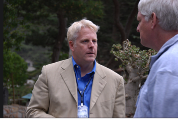
\includegraphics{1.7.png}
\caption{\emph{Lewis Sheperd (izquierda), en ese entonces un alto
funcionario de tecnología de la Agencia de Inteligencia de Defensa del
Pentágono, hablando con Peter Norvig (derecha), renombrado experto en
inteligencia artificial y director de investigaciones de Google. Esta
fotografía es de la reunión del Foro Highlands de 2007}}
\end{figure}

Norvig se muestra en el perfil de Google Plus de O'Neill como uno de sus
contactos cercanos. El alcance del resto de las contactos de O'Neill en
Google Plus ilustra que está directamente conectado no solamente con un
amplio rango de ejecutivos de Google, sino también con los nombres más
importantes de la comunidad de tecnología de EE.UU.

Estas conexiones incluyen a Michele Weslander Quaid, una ex contratista
de la CIA y anterior oficial senior de inteligencia del Pentágono quien
es actualmente directora de tecnología de Google donde está
desarrollando programas que ``se ajusten mejor a las necesidades de las
agencias gubernamentales''; Elizabeth Churchill, director de experiencia
de usuario de Google; James Kuffner, un experto en robótica humanoide
que encabeza la división de robótica de Google y que introdujo el
término ``robótica en la nube''; Mark Drapeau, director de compromiso
para el cambio para los negocios de Microsoft con el sector público;
Lili Cheng, administrador general del Laboratorio de Experiencias
Sociales Futuras de Microsoft (FUSE); Jon Udell, ``evangelista'' de
Microsoft; Cory Ondrejka, vicepresidente de ingeniería de Facebook; para
nombrar solo unos pocos.

En 2010, Google firmó un contrato de adjudicación directa por varios
miles de millones de dólares con la agencia hermana de la NSA, la
Agencia Nacional de Inteligencia Geospacial (NGA). El contrato era para
usar Google Earth para los servicios de visualización de la NGA. Google
ha desarrollado el software detrás de Google Earth al comprar Keyhole de
la empresa de riesgo de la CIA, In-Q-Tel.

Luego un año después, en 2011, otro contacto de O'Neill en Google Plus,
Michele Quaid - quien ha serviso en posiciones ejecutivas en la NGA, en
la Oficina de Reconocimiento Nacional y en la oficina del director de
Inteligencia Nacional - abandonó su rol en el gobierno para convertirse
en una ``evangelista de la innovación'' y la persona señalada para
buscar contratos con el gobierno. La última función de Quaid antes de
partir hacia Google fue como representante principal del Director de
Inteligencia Nacional ante la Fuerza Especial de Inteligencia,
Vigilancia y Reconocimiento, y como asesor principal del subsecretario
de defensa para el director de inteligencia del Conjunto y Coalición de
Apoyo al Combatiente (J\&CWS). Ambos roles involucran operaciones de
información principalmente. Antes de irse a Google, en otras palabras,
Quaid trabajó estrechamente con la Oficina de la Subsecretaría de
Defensa para la Inteligencia, que está subordinada al Foro Highlands del
Pentágono. Quaid ha asistido personalmente al Foro, aunque no pude
confirmar con precisión cuando y con qué frecuencia.

En marzo de 2012, la entonces directora de DARPA Regina Duran - quien
por sus competencias también co-dirigía el Foro Highlands del Pentágono
- siguió a su Colega Quaid a Google para liderar al nuevo Grupo de
Tecnología Avanzada y Proyectos de la compañía. Durante su desempeño en
el Pentágono, Duran encabezó las iniciativas de ciberseguridad
estratégica y redes sociales entre otras. Ella era responsable de
concentrar ``una porción creciente'' del trabajo de DARPA ``en la
investigación de capacidades ofensivas para abordar necesidades
militares específicas'', asegurando 500 millones de dólares del gobierno
para financiar ciber investigaciones de DARPA desde 2012 hasta 2017.

\begin{figure}[htbp]
\centering

\includegraphics{1.8.png}
\caption{\emph{Regina Dugan, ex jefa de DARPA y codirectora del Foro
Highlands, ahora una ejecutiva de alto rango de Google -tratando de
lucir adecuadamente para la ocasión}}
\end{figure}

Por noviembre de 2014, el jefe de IA de Google y experto en robótica
James Kuffner fue un delegado junto con O'Neill al Foro Highlands 2014
en Singapur, para explorar ``Avances en robótica e inteligencia
artificial: implicaciones para la sociedad, la seguridad y el
conflicto''. El evento incluyó 26 delegados de Austria, Israel, Japón,
Singapur, Suecia, Gran Bretaña y EE.UU., tanto de la industria como del
gobierno. La asociación de Kuffner con el Pentágono. sin embargo.
comenzó mucho antes. En 1997, Kuffner fue un investigador durante su
doctorado en Stanford de un proyecto financiado por el Pentágono sobre
robots móviles autónomos en red, patrocinados por DARPA y la marina de
EE.UU.

\subsection{Rumsfeld y la vigilancia
persistente}\label{rumsfeld-y-la-vigilancia-persistente}

Resumiendo, muchos de los ejecutivos más importantes de Google están
asociados con el Foro Highlands del Pentágono, el cual a través del
período de crecimiento de Google por más de una década ha funcionado
repetidamente como una fuerza convocante para establecer conexiones. La
incubación de Google por parte de la comunidad de inteligencia de EE.UU.
desde sus comienzos ocurrió a través de una combinación de patrocinio
directo y de redes informales de influencia financiera, firmemente
alineadas con los intereses del Pentágono

El propio Foro Highlands ha utilizado la construcción de relaciones
informales de tales redes privadas para reunir a los sectores de
industria y defensa, permitiendo la fusión de intereses corporativos y
militares para expandir el aparato de vigilancia encubierto en el nombre
de la seguridad nacional. El poder ejercido por la red oculta
representada en el Foro, sin embargo, puede estimarse más claramente
desde su impacto durante la administración Bush, cuando desempeñó un rol
directo redactando literalmente las estrategias y doctrinas detrás de
los intentos de EE.UU. para conseguir ``superioridad en la
información''.

En diciembre de 2001, O'Neill confirmó que las discusiones estratégicas
del Foro Highlands se estaban alimentando directamente de la revisión
estratégica de Andrew Marshall de todo el DoD ordenado por el Presidente
Bush y Donald Rumsfeld para actualizar las fuerzas armadas, incluyendo
la Revisión Cuatrienal de Defensa - y que algunos de las primeras
reuniones del Foro ``resultaron en la redacción de un grupo de
políticas, estrategias y doctrinas del DoD para los servicios en la
guerra de la información''. El proceso de ``redactar'' las políticas de
la guerra de la información del Pentágono ``fue hecho en conjunto con
las personas que entendieron de otra manera al entorno - no solamente
los ciudadanos estadounidenses, sino también los extranjeros, y las
personas que estaban desarrollando TI corporativa''.

Las doctrinas de la guerra de la información del Pentágono después del
11-S fueron escritas, entonces, no sólo por funcionarios de seguridad
nacional de EE.UU. y en el extranjero: también intervinieron poderosas
entidades corporativas en los sectores de tecnologíia y defensa.

En abril de ese año, el general James McCarthy completó su revisión para
reestructurar el sector de defensa ordenada por Rumsfeld. Su reporte
resaltaba repetidamente la vigilancia global como fundamental para la
transformación del DoD. En cuanto a Marshall, en su informe posterior a
Rumsfeld desarrolló un plan para determinar el futuro del Pentágono en
la ``era de la información''.

O'Ńeill también afirmó que el desarrollar la doctrina de la guerra de la
información, el Foro ha mantenido extensas discusiones acerca de
vigilancia electrónica y ``que constituyen un acto de guerra en un
entorno de información''. Los papers basados en la política de defensa
de los EE.UU. escritos en los primeros años de la década del '90 por los
consultores de RAND John Arquila y David Ronfeldt, ambos miembros
antiguos del Foro Highlands, fueron producidos ``como resultado de
aquellas reuniones'', al explorar los dilemas de la política acerca de
cuánto faltaba para cumplir el objetivo de la ``superioridad en la
información''. Una de las cosas que impactaron al público estadounidense
fue que no estábamos robando electrónicamente las cuentas de Milosevic
cuando de hecho hubiéramos podido hacerlo``, comentó O'Neill

Aunque el proceso de I+D alrededor de la estrategia de transformación
del Pentágono es confidencial, se pueden encontrar indicios de las
discusiones del DoD en ese período en una monografía de investigación
del año 2005 de la Escuela de Estudios Militares Avanzados de la Armada
de EE.UU. en la revista \emph{Military Review}, autorizada por un activo
oficial de inteligencia de la Armada.

``La idea de la Vigilancia Persistente como un potencial de
transformación ha circulado dentro de la Comunidad de Inteligencia (IC)
nacional y el Departamento de Defensa (DoD) durante los últimos tres
años'', decía el paper, en referencia al estudio de reestructuración
encargado por Rumsfeld.

El paper de la Marina hizo una revisión de una variedad de documentos
miiltares oficiales de alto nivel, incluyendo uno de la Oficina del
Presidente del Estado Mayor Conjunto, que muestra que la ``Vigilancia
Persistente'' era un tema fundamental de la visión centrada en la
información para la política de defensa a través del Pentágono.

Ahora sabemos que sólo dos meses antes del discurso de O'Neill en
Harvard 2001, bajo el programa TIA, el presidente Bush autorizó
secretamente la vigilancia doméstica de los estadounidenses sin orden
judicial, en lo que parecía haber sido una modificación ilegal del
proyecto de data mining ThinThread - como fue expuesto posteriormente
por los informantes William Binney y Thomas Drake.

\subsection{El nudo del comienzo de la
vigilancia}\label{el-nudo-del-comienzo-de-la-vigilancia}

A partir de aquí, SAIC, el socio del Foro Highlands, jugó un rol clave
en el despliege de la NSA desde el principio. Poco después del 11-S,
Brian Sharkey, director de tecnología del sector ELS3 del SAIC (enfocado
en los sistemas de TI para sistemas de emergencias), formó equipo con
John Poindexter para proponer el programa de vigilancia TIA. Sharkey de
SAIC había sido previamente subdirector de la Oficina de Sistemas de
Información de DARPA durante la década del '90.

Mientras tanto, por el mismo tiempo, el vicepresidente de SAIC para el
desarrollo corporativo, Samuel Visner, se convirtió en el jefe de los
programas de inteligencia de señales de la NSA. SAIC fue una de las
corporaciones que recibió un contrato por 280 millones de dólares para
desarrollar uno de los sistemas de espionaje secretos de la NSA. En
2003, Visner retornó a SAIC para convertirse en el director de
planeamiento y desarrollo de negocios del grupo de inteligencia de la
empresa.

Ese año, la NSA consolidó su programa TIA de vigilancia electrónica sin
orden judicial, para ``monitorear a los individuos'' y comprender ``cómo
encajan dentro de los modelos'' a través de los perfiles de riesgo de
los ciudadanos estadounidenses y de los extranjeros. TIA estaba haciendo
esto integrando bases de datos de finanzas, de viajes, médicas,
educativas y otros registros dentro de una ``gran base de datos virtual
centralizada''.

Esto sucedió también en el año en que la administración Bush elaboró su
famoso hoja de ruta de las Operaciones de Información (IO) . Al
describir a Internet como un ``sistema de armas vulnerable'', la hoja de
ruta de las IO de Rumsfeld propuso que la estrategia del Pentágono
``debería estar basada en la premisa de que el DoD `combatirá a la red'
como si fuera un sistema de armas enemigo''. EE.UU. debería buscar el
``máximo control'' del ``espectro completo de los sistemas de
comunicaciones emergentes, sensores y sistemas de armas'', según propone
el documento.

Al año siguiente, John Poindexter, que había propuesto y ejecuta el
programa de vigilancia de TIA por medio de su puesto en DARPA, estaba en
Singapur participando en el Foro Island de Highlands 2004. Otros
delegados incluyeron entonces al presidente adjunto del Foro Highlands y
CIO del Pentágono Linton Wells, el presidente del famoso contratista de
la guerra de la información del Pentágono, John Rendon; Karl Lowe,
director del Comando de Fuerzas Conjuntas (JFCOM) de la División Mixta
de Guerra Avanzada; el general de división de la fuerza aérea Stephen
Dalton, el administrador de capacidades para la superioridad de la
información en el Ministerio de Defensa del Reino Unido; Tte Gral. Johan
Kihl, el Jefe del Estado Mayor Comandante Supremo del Cuartel General
del Ejército Sueco, entre otros.

Como en el 2006, SAIC ha sido premiado con un contrato de la NSA
multimillonario en dólares para desarrollar un gran proyecto de data
mining llamado ExecuteLocus, a pesar del colosal fracaso de 1000
millones de dólares del contrato anterior conocido como ``Trailblazer''.
Los componentes principales de TIA fueron ``tranquilamente continuados''
con ``diferentes alias'', según Política Exterior de Shane Harris, pero
han sido ocultados ``detrás del velo de un presupuesto de inteligencia
confidencial''. El nuevo programa de vigilancia había sido para entonces
desplazado de la oŕbita de DARPA y puesto bajo jurisdicción de la NSA.

Este fue también el año de otro Foro Island en Singapur, conducido por
Richard O'Neill en nombre del Pentágono, que incluyó a funcionarios de
alto rango de la industria y de defensa desde EE.UU, Reino Unido, India
e Israel. Los participantes también incluyeron tecnólogos experimentados
de Microsoft e IBM así como Gilman Louie, socio de la firma de
inversiones en tecnología Alsop Louie Partners.

Gilman Louie es un ex CEO de In-Q-Tel - la firma de la NSA que invierte
especialmente en empresas jóvenes que desarrollan tecnologías de data
minig. In-Q-Tel fue fundada en 1999 por la Dirección de Ciencia y
Tecnología de la CIA, en virtud de la cual operaba la Oficina de
Investigación y Desarrollo (ORD), que era parte del programa financiado
de Google MDSS. La idea fue reemplazar esencialmente las funciones
anteriormente desempeñadas por ORD, al movilizar al sector privado para
desarrollar soluciones de tecnología de información para la comunidad
entera de inteligencia.

Louie lideró In-Q-Tel desde 1999 hasta enero de 2006 - incluso cuando
Google compró Keyhole, el software de mapeo satelital financiado por
In-Q-Tel. Entre sus colegas en la junta de In-Q-Tel en este período
estaban la ex directora de DARPA y copresidenta del Foro Highlands Anita
Jones (aún en el cargo), así como el miembro fundador William Perry: el
hombre señalado por O'Neill para formar el Foro Highlands por primera
vez. Uniéndose a Perry como miembro fundador de In-Q-Tel estaba John
Seely Brown, por entonces jefe científico de Xerox Corp. y director de
su Centro de Investigación Palo Alto (PARC) desde 1990 hasta 2002, que
también es un antiguo miembro del Foro Highlands desde su nacimiento.

Además de la CIA, In-Q-Tel también ha sido respaldado por el FBI, NGA y
la Agencia de Inteligencia de Defensa, entre otras agencias. Más del
60\% de las inversiones de In-Q-Tel supervisadas por Louie eran ``en
empresas especializadas en recolección automática, filtrado y
comprensión de océanos de información'', según News21 de la Escuela
Medill de Periodismo, que observa también que el propio Louie había
reconocido que no estaba claro si la privacidad y las libertades civiles
estarán protegidas" del uso gubernamental de estas tecnologías ``por
razones de seguridad nacional''.

La transcripción del seminario de Richard O'Neill a finales de 2001 en
Harvard muestra que el Foro Highlands del Pentágono tuvo como invitado a
Gilman Louie mucho antes que el Foro Island, de hecho, poco después del
11-S, donde exploró ``qué está sucediendo con In-Q-Tel''. Esta sesión
del Foro enfocada a ``cómo sacar ventaja de la velocidad del mercado
comercial que no está presente dentro de la ciencia y de la comunidad
tecnológica de Washington'' y para comprender ``las implicaciones para
el DoD en términos de la revisión estratégica, el QDR, la acción Hill, y
los accionistas''. Los participantes del encuentro incluyeron
``militares de alto rango'', mandos de combate, ``varios oficiales de
alto rango de la Marina'', algunas ``personas de la industria de
defensa'' y varios congresistas estadounidenses incluyendo el diputado
republicano William Mac Thornberry y el senador demócrata Joseph
Lieberman.

Tanto Thornberry como Lieberman son devotos defensores de la vigilancia
de la NSA, y han actuado en consecuencia para conseguir apoyos para la
legislación pro guerra y pro vigilancia. Los comentarios de O'Neill
indican que el papel del Foro no era solamente permitir que los
contratistas corporativos escriban las políticas del Pentágono, sino
conseguir apoyo político para las políticas gubernamentales adoptadas a
través de la marca informal del Foro de las redes en las sombras.

Repetidamente, O'Neill le relató a su audiencia en Harvard que su
trabajo como presidente del Foro era encontrar casos de estudio de
empresas reales a través del sector privado, como eBay y Human Genome
Science, para plantear la base de la ``superioridad en la información''
estadounidense - ``como dominar'' al mercado de la información - e
influenciarlo para ``que el presidente y el secretario de defensa puedan
hacer lo que deseen con respecto a la transformación del DoD y la
revisión estratégica''.

En 2007, un año después de la reunión del Foro Island que incluyó a
Gilman Louie, Facebook recibió su segundo ronda de \$12.7 millones
financiados por Accel Partners. Accel estaba encabezada por James
Breyer. ex jefe de la Asociación Nacional de Capital de Riesgo (NVCA)
donde Louie también trabajó en la junta mientras era CEO de In-Q-Tel.
Tanto Louie como Breyer han trabajado juntos previamente en la junta de
BBN Technologies - que ha contratado a la ex jefa de DARPA y consejera
de In-Q-Tel Anita Jones.

La ronda 2008 de financiación de Facebook fue liderada por Greylock
Venture Capital, que invirtió 27.5 millones de dólares. Los socios
principales de la empresa incluyen a Howard Cox, otro ex jefe de NVCA
que se sienta en la junta de In-Q-Tel. Además de Breyer y Zuckerberg, el
otro miembro de la junta de Facebook es Peter Thiel, cofundador del
contratista de defensa Palantir que provee toda clase de tecnologías de
visualización y data mining para el gobierno, los militares y las
agencias de inteligencia de EE.UU., incluyendo a la NSA y el FBI, y que
a su vez se alimentó de la viabilidad financiera de los miembros del
Foro Highlands.

Los cofundadores de Palantir Thiel y Alex Karp se reunieron con John
Poindexter en 2004, según Wired, el mismo año en que Poindexter visitó
el Foro Island en Singapur. La reunión tuvo lugar en la casa de Richard
Perle, otro acólito de Andrew Marshall. Poindexter ayudó a Palantir
abriéndole puertas, y presentándole ``una legión de abogados de los
estratos más influyentes del gobierno''. Thiel también se reunió con
Gilman Louie de In-Q-Tel, para asegurarse el respaldo de la CIA en esta
fase temprana.

Y así cerramos el círculo. Los programas de data mining como
ExecuteLocus y sus proyectos relacionados, que fueron desarrollados
durante este período, aparentemente sentaron las bases para los nuevos
programas de la NSA eventualmente revelados por Snowden. En 2008,
Facebook recibió su próxima ronda de financiamiento de Greylock Venture
Capital; como lo confirman los documentos y el testimonio del
denunciante la NSA efectivamente resucitó el proyecto TIA con foco en
data mining en Internet por medio del monitoreo completo de los mensajes
de correo electrónico, los mensajes de texto y la navegación web.

También sabemos ahora gracias a Snowden que el sistema de explotación
``Inteligencia en Red Digital'' XKeyscore de la NSA fue diseñado para
permitirle a los analistas buscar no sólo en las bases de datos de
Internet como los correos electrónicos, los chats online y el historial
de navegación, sino también los servicios telefónicos, audios de
teléfonos móviles, transacciones financieras y comunicaciones de
transportes aéreos globales - esencialmente la red entera de
telecomunicaciones globales. El socio del Foro Highlands, SAIC,
desempeñó un rol clave, entre otros contratistas, en producir y
administrar XKeyscore de la NSA, y estuvo recientemente implicado en el
hacking de la NSA de la red privada Tor.

El Foro Highlands del Pentágono estuvo por lo tanto íntimamente
involucrado en todo esto como una red convocante - pero también muy
directamente. Al confirmar su rol de pivot en la expansión de los
aparatos de vigilancia global liderados por EE.UU., el entonces
copresidente del Foro, CIO del Pentágono Linton Wells, le contó a la
revista FedTech en 2009 que él había supervisado la introdución de la
NSA de ``una impresionante arquitectura a largo plazo el verano pasado
que suministrará seguridad cada vez más sofisticada hasta el 2015 o
más''.

\subsection{La conexión Goldman
Sachs}\label{la-conexiuxf3n-goldman-sachs}

Cuando le pregunté a Wells acerca de la influencia del Foro en la
vigilancia global de EE.UU., respondió que prefería no hacer comentarios
al respecto y que ya no lideraba al grupo.

Aunque Wells ya no está en el gobierno - esto era de esperar - aún está
conectado a Highlands. En septiembre de 2014, después de distribuir su
influyente libro blanco acerca de la transformación del Pentágono, se
unió al Instituto Monterrey para Estudios Internacionales (MIIS)
Iniciativa Ciberseguridad (CySec) como un distinguido y experimentado
investigador.

Desgraciadamente, esto no fue suficiente para mantenerlo ocupado en su
retiro. El cambio de Wells enfatiza la idea del Pentágono de que la
guerra de la información no se relaciona solamente con la vigilancia,
sino también con la explotación de la vigilancia para influir tanto en
el gobierno como en la opinión pública.

La iniciativa MIIS CySec está actualmente asociada con el Foro Highlands
del Pentágono a través del memorándum de entendimiento (MoU) firmado con
la directora del MIIS Dra. Amy Sans, que es miembro del Consejo Asesor
de Seguridad Internacional de la Secretaría de Estado. El sitio web del
MIIS CySec declara que el MoU firmado por Richard O'Neill:

\begin{quote}
\emph{``allana el camino para la futuras sesiones conjuntas MIIS
CySec-Grupo Highlands que explorarán el impacto de la tecnología sobre
la seguridad, la paz y el compromiso de la información. Durante
alrededor de 20 añosel Grupo Highlands se ha comprometido con el sector
privado y los líderes gubernamentales, incluyendo al Director Nacional
de Inteligencia, DARPA, la oficina del secretario de defensa, la oficina
del secretario de seguridad nacional y el ministro de defensa de
Singapur, en conversaciones productivas para enmarcar las áreas de
política y de tecnología.''}
\end{quote}

¿Quién es el benefactor financiero de la nueva iniciativa de asociación
entre Highlands del Pentágono y MIIS CySec? Según el sitio web de MIIS
CySec, la iniciativa fue lanzada ``a través de una generosa donación de
capital inicial de George Lee''. George C. Lee es un socio principal de
Goldman Sachs, donde es el CIO de la división de inversiones bancarias,
y jefe del grupo de Medios, Telecomunicaciones y Tecnología Global
(TMT).

Pero hay algo más. En 2011, fue Lee quien construyó la valuación de 50
mil millones de dólares de Facebook, y previamente había hecho tratos
para otros gigantes conectados a Highlands tales como Google, eBay y
Microsoft. El entonces jefe de Lee, Stephen Friedman, un ex CEO y
director de Goldman Sachs, y posteriormente socio principal en la mesa
directiva de la firma, fue también un miembro fundador de la junta
directiva de In-Q-Tel junto al jefe supremo William Perry y al miembro
del Foro Seely Brown.

En 2001, Bush incorporó a Stephen Friedman al Consejo Asesor de
Inteligencia del Presidente, quien lo dirigió desde 2005 hasta 2009.
Friedman había trabajado previamente junto a Paul Wolfowitz y otros
durante 1995-1996 en la comisión presidencial de investigación de
competencias en inteligencia de EE.UU, y en 1996 enel Panel Jeremiah con
Martin Faga, el vicepresidente senior y administrador general del Centro
Corporativo para Sistemas de Inteligencia Integrados de MITRE - donde
Thuraisingham, que administró el programa de la CIA-NSA-MDDS que inspiró
el data mining contraterrorista DARPA, fue también un ingeniero
principal.

En las notas al pie de un capítulo para el libro, \emph{Ciberespacio y
Seguridad Nacional} (Georgetown University Press), el ejecutivo de
SAIC/Leidos Jeff Cooper revela que otro socio principal de Goldman
Sachs, Philip J. Venables - que como director de riesgos de la
información lideró los programas de la empresa sobre seguridad de la
información - desarrolló una presentación en el Foro Highlands 2008
llamada \emph{Sesión de fortalecimiento de la disuasión}. El capítulo de
Cooper recurrió a la presentación en Highlands ``tras pedirle
autorización''. En 2010, Venables participó con su entonces jefe
Friedman en una reunión en el Instituto Aspen sobre la economía mundial.
Durante los últimos años, Venables también participó de varias
comisiones evaluadoras de premios de ciberseguridad de la NSA.

En síntesis, la firma de inversión responsable de crear las fortunas de
miles de millones de dólares de las sensaciones de la tecnología del
siglo XXI, desde Google a Facebook, está íntimamente relacionada con la
comunidad de inteligencia militar de EE.UU.; con Venables, Lee y
Friedman ya sea directamente conectados al Foro Highlands del Pentágono,
o a los miembros principales del Foro.

\subsection{Combatiendo al terror con
terror}\label{combatiendo-al-terror-con-terror}

La confluencia de estos poderosos intereses financieros y militares
alrededor del Foro Highlands, por medio del patrocinio de George Lee al
nuevo socio del Foro, la iniciativa MIIS CySec, en relevante por si
misma.

La directora de MIIS CySec, la Dra. Itamara Lochard, ha estado inmersa
en Highlands. Ella regularmente ``presenta investigaciones actuales
sobre grupos no gubernamentales, gobernanza, tecnología y conflictos a
la oficina del secretario de defensa de EE.UU Foro Highlands'', de
acuerdo a au biografía en la Universidad Tutfs. También ``habitualmente
asesora a los mandos de combate estadounidenses'' y se especializa en
estudiar el uso de la tecnología de la información de los ``grupos
subestatales violentos y no violentos''.

\begin{figure}[htbp]
\centering
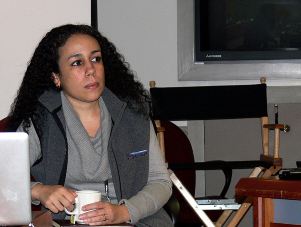
\includegraphics{1.9.png}
\caption{\emph{La Dra. Itamara Lochard es un miembro destacado del Foro
Highlands y experta en información del Pentágono. Ella dirige la
iniciativa CyberSec del MIIS que ahora apoya al Foro Highlands del
Pentágono con financiamiento del socio de Goldman Sachs, George Lee, que
lideró las tasaciones de Facebook y Google}}
\end{figure}

La Dra. Lochard mantiene una base de datos completa de 1700
organizaciones no gubernamentales incluyendo ``insurgentes,
paramilitares, terroristas, complejas organizaciones criminales, bandas
organizadas, ciber actores sociales, actores sociales no violentos
estratégicos'', para analizar sus ``patrones de organización, áreas de
cooperación, estrategias y tácticas''. Preste atención, aquí, a la
mención de ``actores sociales no violentos estratégicos'' - los cuales
quizás abarca a las ONG y otros grupos u organizaciones comprometidas en
la actividad o campaña política, a juzgar por el foco de otros programas
de investigación del DoD.

Desde el 2008. Lochard ha sido una profesora adjunta de la Universidad
de Operaciones Especiales Conjuntas de los EE.UU. donde dictaba un curso
avanzado top secret en ``Guerra irregular'' que ella diseñó para los
oficiales superiores de las fuerzas especiales de EE.UU. Previamente
había dictado cursos en ``Guerra interna'' para ``oficiales
político-militares'' de alto rango de varios regímenes del Golfo.

Sus puntos de vista revelan por lo tanto mucho acerca de lo que el Foro
Highlands ha estado asesorando en todos estos años. En 2004, Lochard fue
coautora de un estudio para el Instituto de Estudios de Seguridad
Nacional de la Fuerza Aérea de los EE.UU. sobre las estrategias
estadounidenses más allá de las ``organizaciones no gubernamentales
armadas''. El estudio por un lado sostenía que los grupos armados no
gubernamentales deberían ser reconocidos con urgencia como la
``prioridad de seguridad número uno'', y por el otro que la
proliferación de grupos armados ``brinda oportunidades estratégicas que
pueden ser explotadas para ayudar a alcanzar las metas políticas.
Existen y existirán casos donde EE.UU. encuentre que colaborar con
grupos armados sea beneficioso para sus intereses estratégicos''. Pero
se deben desarrollar ``herramientas sofisticadas'' para diferenciar los
grupos y comprender sus dinámicas, para determinar cuáles deberían ser
neutralizados y cuáles explotados en beneficio de EE.UU. ``Los perfiles
de los grupos armados pueden asimismo ser empleados para identificar las
formas en las cuales EE.UU. pueda ayudar a algunos de ellos y cuyo éxito
será beneficioso para los objetivos políticos de EE.UU. en el
extranjero''.

En 2008 Wikileaks publicó una filtración de un manual de campo de las
Operaciones Especiales de la Armada de EE.UU. de acceso restringido, que
demostraba que la clase de ideas defendidas por la experta de Highlands
Lochard han sido explícitamente adoptadas por las fuerzas especiales de
EE.UU.

El trabajo de Lochard demuestra que el Foro Highlands está situado en la
intersección de la estrategia avanzada del Pentágono sobre vigilancia,
operaciones encubiertas y guerra irregular: ya sea movilizando la
vigilancia global para desarrollar información detallada sobre grupos
violentos y no violentos percibidos como potencialmente amenazantes para
los intereses de EE.UU., u ofreciendo oportunidades de explotarla,
alimentándose directamente de sus operaciones encubiertas.

Esto último es la razón por la cual la CIA, la NSA y el Pentágono
engendraron Google: para poder ejecutar sus guerras sucias secretas con
una eficiencia nunca antes vista. \#\# Dentro de la red secreta detrás
de la vigilancia global, una guerra sin fin, y Skynet - parte II

La vigilancia global se refiere al control. Quienes la impulsan pueden
reclamar, incluso creer, que el control es por el bien común, y que es
necesario para mantener el orden, para estar totalmente preparado para
enfrentar la pŕoxima amenaza. Pero en un contexto de corrupción política
rampante, crecientes desigualdades económicas, y la escalada de la
escasez de recursos debido al cambio climático y a la volatilidad de la
energía, la vigilancia global puede convertirse en una herramienta del
poder para autoperpetuarse, a expensas de la población.

Una de las funciones principales de la vigilancia global que ha menudo
se pasa por alto es conocer al adversario a tal punto que pueda ser
manipulado hasta doblegarlo. El problema es que el adversario no son
sólo los terroristas. Somos usted y yo. En la actualidad, el papel de la
guerra de la información como propaganda está en pleno apogeo, aunque es
sistemáticamente ignorado por muchos de los medios de comunicación.

Aquí, INSURGE INTELLIGENCE expone cómo la cooptación por parte del Foro
Highlands del Pentágono de gigantes de la tecnología como Google en pos
de la vigilancia global, ha jugado un rol clave en los esfuerzos
secretos para manipular los medios de comunicación como parte de una
guerra de la información en contra del gobierno de EE.UU., los
estadounidenses y el resto de las personas del mundo: la justificación
de la guerra sin fin, y un continuo expansionismo militar.

\subsection{La máquina de guerra}\label{la-muxe1quina-de-guerra}

En septiembre del 2013, el sitio web de la Iniciativa de Ciberseguridad
para los Estudios Internacionales del Instituto Monterey (MIIS CySec)
publicó una versión final del paper sobre ``ciber-disuasión'' del
consultor de la CIA Jeffrey Cooper, vicepresidente de la empresa SAIC,
contratista de defensa de Estados Unidos, y miembro del Foro Highlands
del Pentágono. El paper fue presentado al entonces director de la NSA
general Keith Alexander en la sesión del Foro Highlands titulada ``Los
bienes ciber-comunes, enfrentamientos y disuasión'' en 2010.

\begin{figure}[htbp]
\centering
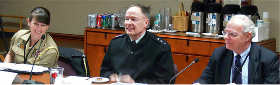
\includegraphics{2.1.png}
\caption{\emph{Gral. Keith Alexander (centro), quien se desempeñó como
director de la NSA y jefe del Servicio Central de Seguridad de 2005 a
2014, y también como comandante del Cibercomando de Estados Unidos de
2010 a 2014, en la sesión de 2010 sobre ciber-disuasión del Foro
Highlands}}
\end{figure}

MIIS CySec está formalmente asociada al Foro Highlands del Pentágono a
través de un memorándum de entendimiento firmado entre el decano y el
presidente del Foro Richard O'Neill, mientras la iniciativa misma fue
fundada por George C. Lee, el ejecutivo de Goldman Sachs que condujo a
las valuaciones de miles de millones de dólares de Facebook, eBay y
Google, entre otras empresas.

El paper revelador de Cooper no está más disponible en el sitio web del
MIIS, pero se puede hallar una versión final por medio de los registros
de una conferencia pública de seguridad nacional alojada en el Colegio
de Abogados de Estados Unidos. En la actualidad, Cooper es el director
de innovación de SAIC/Leidos, que es parte integrante de un consorcio de
empresas de tecnología de defensa que incluye a Booz Allen Hamilton
entre otros contratistas para perfeccionar la capacidad de vigilancia de
la NSA.

La presentación del Foro Highlands para el jefe de la NSA fue contratada
por el subsecretario de defensa para la inteligencia, y basada en los
conceptos desarrollados en las reuniones previas del Foro. Esta sesión
se le presentó al gral. Alexander como una ``sesión cerrada'' del Foro
Highlands moderada por la directora del MIIS CySec, Dra. Itamara
Lochard, en el Centro para Estudios Internacionales y Estratégicos
(CSIS) en Washington DC.

\begin{figure}[htbp]
\centering
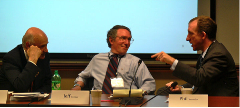
\includegraphics{2.2.png}
\caption{\emph{Jeffrey Cooper de SAIC/Leidos (centro), uno de los
miembros fundadores del Foro Highlands del Pentágono, escuchando a Phil
Venables (derecha), socio principal de Goldman Sachs, en la sesión de
2010 del Foro sobre ciber-disuasión en la CSIS}}
\end{figure}

Como guía de las operaciones de información de Rumsfeld, las sesiones
informativas de la NSA de Cooper describieron a los ``sistemas de
información digital'' tanto como una ``enorme fuente de vulnerabilidad''
como ``armas y herramientas poderosas'' para la ``seguridad nacional''.
También insistió en la necesidad de que la ciber inteligencia de Estados
Unidos amplíe el ``profundo conocimiento'' de los adversarios
potenciales y reales, para poder identificar ``cada objetivo
estratégico'' que pueda ser explotado para la disuasión o la represalia.
La ``disuasión en red'' requiere que la comunidad de inteligencia de
Estados Unidos desarrolle una ``profunda comprensión y un conocimiento
específico acerca de las redes involucradas y sus patrones de enlaces,
incluyendo sus tipos y su intensidad'' además de usar a las ciencias
cognitivas y del comportamiento para poder predecir patrones. Su paper
esencialmente sentó las bases de la arquitectura teórica del modelado de
datos obtenidos a partir de la vigilancia y las redes sociales sobre
lospotenciales ``adversarios'' y los ``amigos''.

Un año después de la presentación con el director de la NSA, Michele
Weslander Quaid - otro delegado del Foro Highlands - se unió a Google
para convertirse en el Director de Tecnología, manteniendo su alto cargo
en el Pentágono asesorando al subsecretario de defensa para la
inteligencia. Dos meses antes, el Consejo Científico de Defensa (DSB)
Grupo de Trabajo sobre Inteligencia de Defensa publicó su informe sobre
Operaciones de Contrainsurgencia (COIN), Inteligencia, Vigilancia y
Reconocimiento (IRS). Quaid estuvo entre los expertos de inteligencia
del gobierno que aconsejaron e informaron al Grupo de Trabajo Consejo
Científico de Defensa en la preparación del informe. Otro experto que
asesoró al Grupo de Trabajo fue el veterano del Foro Highlands Linton
Wells. El propio informe del DSB ha sido encargado por un hombre de
Bush, James Clapper, el subsecretario de defensa para inteligencia - que
también encargó la presentación de Cooper en el Foro Highlands al gral.
Alexander. Clapper es el actual Director de Inteligencia Nacional de
Obama, el mismo que mintió bajo juramento al Congreso de EE.UU. en marzo
de 2013 al declarar que la NSA no recopila ningún dato sobre los
ciudadanos estadounidenses.

Michele Quaid registra un paso a través de la comunidad de inteligencia
militar estadounidense en la transición de las agencias en el uso de
herramientas web y tecnología de nube. La impronta de sus ideas son
evidentes en las partes principales del informe del Grupo de Trabajo
OSD, que describe su propósito como ``influenciar en las decisiones de
inversión'' en el Pentágono ``recomendando las aptitudes apropiadas para
la comunidad de inteligencia que le posibiliten evaluar las
insurgencias, comprender una población en su entorno, y apoyar las
operaciones de contrainsurgencia''.

El informe menciona 24 países del sur y del sudeste de Asia, del norte y
del oeste de Africa, Oriente Medio y Sudamérica, quienes podrían
plantear ``posibles desafíos insurgentes'' para los militares de Estados
Unidos en los años venideros. Algunos de los países incluidos son
Pakistán, México, Yemen, Nigeria, Guatemala, Gaza/Cisjordania, Egipto,
Arabia Saudita y Líbano, entre otros ``regímenes autocráticos''. El
informe aduce que ``la crisis económica, el cambio climático, las
presiones demográficas, la escasez de recursos, o un mal gobierno
podrían llevar a estos estados (u otros) a la quiebra o debilitarse
tanto que se podrían convertir en objetivos para los agresores y/o
insurgentes''. A partir de ahí, la ``infraestructura de información
global'' y los ``medios sociales'' pueden rápidamente ``amplificar la
velocidad, intensidad y el momento de los sucesos'' con implicaciones
regionales. ``Esas zonas podrían convertirse en refugios a partir del
cual lanzar ataques al suelo estadounidense, reclutar adeptos, y
financiar, entrenar y abastecer sus operaciones''.

Lo primordial en este contexto es incrementar la capacidad militar de
las operaciones de ``disuasión'' - evitando una intervención mayor de
las fuerzas armadas - para evitar las insurgencias, o anticiparse a
ellas cuando aún se encuentran en su estado incipiente. El informe
concluye que ``Internet y los medios sociales son las fuentes
fundamentales de datos para el análisis de redes sociales en las
sociedades que no solo saben leer y escribir, sino también conectarse a
Internet''. Esto requiere ``monitorear la blogósfera y otros medios
sociales a través de muchas diversas culturas y lenguajes'' para
prepararse para las ``operaciones centradas en la operación''.

El Pentágono también debe incrementar su capacidad para ``modelar y
simular el comportamiento'' para una ``mejor comprensión y anticipación
de las acciones de la población'' basadas en los ``datos obtenidos de
las poblaciones, redes humanas y geográficas, y otras características
económicas y sociales''. Dichas ``operaciones centradas en la
población'' también serán ``cada vez más'' necesarias en ``conflictos
por recursos emergentes, ya sean basados en la crisis del agua, el
agotamiento de la agricultura, del medio ambiente, o los dividendos'' de
los recursos minerales. Esto debe incluir el monitores de la
``demografía de la población como una parte orgánica en el marco de los
recursos naturales''.

Otras áreas donde se debe poner más atención son la ``video vigilancia
aérea'', los ``datos sobre terreno de alta resolución'', la ``capacidad
de computación en la nube'' y la ``fusión de datos'' para todas las
formas de inteligencia en un ``marco espacio-temporal coherente para
organizar e indexar los datos'', desarrollando los ``marcos de las
ciencias sociales'' que pueda ``soportar la codificación y el análisis
espacio-temporal'', la ``distribución de tecnologías de autenticación
biométrica multiforme (''como huellas digitales, escáneres de retina y
muestras de ADN``) para mejorar procesos administrativos básicos'' para
``identificar a cada individuo que realice una transacción''. Además, la
academia debe ayudar al Pentágono a obtener ``muchos tipos diferentes de
datos e información de las ciencias sociales y del comportamiento, entre
ellos datos humanos antropológicos, socio-culturales, históricos,
geográficos, educativos y de salud pública'' para desarrollar ``una
profunda comprensión de las poblaciones''.

Pocos meses después de unirse a Google, Quaid representó a la empresa en
agosto de 2011 en el foro de industria y clientes de la Agencia de
Sistemas de Información de Defensa (DISA) del Pentágono. El foro debía
proveer a ``los servicios, fuerzas de combate, agencias y fuerzas de
coalición'' la ``oportunidad para relacionarse directamente con la
industria de tecnologías innovadoras para dotar y mejorar las
capacidades en apoyo de nuestros combatientes''. Los participantes del
evento fueron una parte esencial en los esfuerzos para crear un
``entorno de información empresarial para la defensa'', definido como
``una plataforma integrada que incluye la red, la informática, el
entorno, los servicios, el aseguramiento de la información y las
capacidades de hacer operaciones en la red'', permitiéndole a los
combatientes ``conectarse, autenticarse, descubrir y compartir
información y colaborar a través del espectro completo de las
operaciones militares''. La mayoría de los panelistas del foro eran
funcionarios del departamento de defensa de Estados Unidos, excepto
cuatro, uno de los cuales era Quaid de Google.

Los funcionarios de DISA han asistido también al Foro Highlands - por
ejemplo Paul Friedrichs, director técnico y jefe de ingenieros de la
Oficina del Jefe Ejecutivo de Seguridad de la Información de DISA.

\subsection{Conocimiento es poder}\label{conocimiento-es-poder}

En vista de lo anterior no sorprende que en 2012, pocos meses después
que la codirectora del Foro Highlands dejara DARPA para unirse a Google
como ejecutivo senior, el entonces director de la NSA, gral. Keith
Alexander enviara un mensaje de correo electrónico al fundador y
ejecutivo de Google Sergey Brin para discutir acerca de cómo compartir
información por la seguridad nacional. En aquellos mensajes, obtenidos
bajo la ley de libertad de información por el periodista de
investigación Jason Leopold, el gral. Alexander describió a Google como
un ``miembro clave de la base industrial de defensa (militar de Estados
Unidos)'', una posición que Michele Quaid aparentemente estaba
consolidando. La relación jovial de Brin con el director de la NSA ahora
queda perfectamente en claro dado que Brin ha estado en contacto con los
representantes de la CIA y la NSA, quienes en parte financiaron y
supervisaron su creación del motor de búsqueda de Google, desde mediados
de los '90.

En julio de 2014, Quaid habló con el mando del ejército de Estados
Unidos sobre la creación de una ``célula de adquisición rápida'' para
potenciar sus ``ciber-capacidades'' como parte de la iniciativa de
transformación 2025 de la fuerza. Ella le dijo a funcionarios del
Pentágono que ``muchos de los objetivos tecnológicos del ejército para
el año 2025 podrán concretarse con tecnología comercial ya disponible o
en vías de desarrollo'', reafirmando que ``la industria está preparada
para acompañar al ejército apoyando el nuevo paradigma''. Por esos días,
la mayoría de los medios de comunicación vociferaban la idea de que
Google estaba tratando de distanciarse de la financiación del Pentágono,
pero en realidad, Google ha cambiado sus tácticas para desarrollar
independientemente tecnologías comerciales que tendrían aplicaciones
militares para lograr las metas de transformación del Pentágono.

Sin embargo Quaid no es la única responsable de la relación de Google
con la comunidad de inteligencia militar de Estados Unidos.

En 2004, un año después de que Google comprara el software de mapeo
Keyhole de In-Q-Tel, la empresa de capital de riesgo de la CIA, el
director de evaluación técnica de In-Q-Tel Rob Painter - quien desempeñó
un rol clave en la inversión en primer lugar de In-Q-Tel en Keyhole -
pasó a Google. El trabajo de Painter en In-Q-Tel estaba enfocado en la
identificación, investigación y evaluación de ``empresas emergentes de
nuevas tecnologías que estimamos pueden ser de enorme valor para la CIA,
la Agencia Geoespacial de Inteligencia Nacional (NGA), y la Agencia de
Inteligencia de Defensa''. Además, la NGA confirmó que su inteligencia
obtenida a partir de Keyhole fue usada por la NSA para apoyar
operaciones de Estados Unidos en Irak desde el año 2003 en adelante.

El nuevo trabajo de Painter, un ex funcionario de inteligencia de
operaciones especiales del ejército de EE.UU., fue en Google desde julio
de 2005, como administrador federal de aquello en lo que Keyhole se
convertiría: el emprendimiento Google Earth. En 2007, Painter ya era
jefe de tecnología federal de Google.

Ese año, Painter le contó a \emph{The Washington Post} que Google estaba
``en su etapa inicial'' de venta de versiones secretas avanzadas de sus
productos al gobierno de EE.UU. ``Google ha incrementado su equipo de
ventas en el área de Washington el año pasado para adaptar sus productos
tecnológicos a las necesidades de las agencias civiles y militares y de
la comunidad de inteligencia'' reportaba el Post. El Pentágono ya estaba
usando una versión de Google Earth desarrollada en conjunto con Lockheed
Martin para ``mostrar información a los militares sobre el terreno en
Iraq'', incluyendo ``la ubicación en pantalla de las regiones claves del
país'' y un bosquejo de ``los vecindarios sunita y chiita en Baghdad,
así como de las bases militares estadounidenses e iraquíes en la ciudad.
Ni Lockheed ni Google dijeron como usa los datos la agencia
geoespacial''. Google pretendió venderle al gobierno nuevas ``versiones
mejoradas de Google Earth'' y ``motores de búsqueda para que puedan ser
usados internamente por las agencias''

Los documentos de la Casa Blanca filtrados en 2010 mostraron que los
ejecutivos de Google mantuvieron varias reuniones con funcionarios de
alto rango del Consejo de Seguridad Nacional de Estados Unidos Alan
Davidson, director de asuntos con el gobierno de Google, mantuvo al
menos tres reuniones con funcionarios del Consejo de Seguridad Nacional
en 2009, incluyendo el director principal para asuntos con Rusia de la
Casa Blanca Mike McFault y el asesor sobre Medio Oriente Daniel Shapiro.
Esto también se observa en la aplicación de la patente de Google que la
empresa deliberadamente ha estado recopilando datos ``de carga útil'' de
redes inalámbricas privadas que permitirían la identificación de
``geolocalizaciones''. El mismo año, ahora lo sabemos, Google firmó un
acuerdo con la NSA que le permitía a la agencia un acceso ilimitado a la
información personal de sus usuarios, su hardware y su software, en el
nombre de la ciberseguridad - acuerdo que mantuvo ocupado al gral.
Alexander reproduciéndolo con los CEOs de las empresas de
telecomunicaciones alrededor del país.

Aunque Google es un colaborador clave, base del complejo
militar-industrial estadounidense, no es el único: es toda la Internet y
la amplia gama de empresas del sector privado - muchas nutridas y
financiadas bajo el manto de la comunidad de inteligencia de Estados
Unidos (o por poderosos financistas inmersos en esa comunidad) - que
sostienen la Internet y la infraestructura de telecomunicaciones;
también es la miríada de empresas incipientes que venden tecnologías
innovadoras a la empresa de riesgo de la CIA, In-Q-Tel, donde pueden ser
adaptadas y mejoradas para ser aplicadas en toda la comunidad de
inteligencia militar. En definitiva, el aparato de vigilancia global y
las herramientas secretas utilizadas por agencias como la NSA para
administrarlo, han sido hechas casi en su totalidad por investigadores
externos y contratistas privados como Google, que operan fuera del
Pentágono.

Esta estructura, reflejada en el funcionamiento del Foro Highlands, le
permite al Pentágono capitalizar rápidamente las innovaciones
tecnológicas que de otra manera se perderían, manteniendo al mismo
tiempo los brazos abiertos al sector privado, al menos en apariencia,
para evitar preguntas incómodas acerca de cómo está siendo utilizada
dicha tecnología.

Pero, ¿no es obvio, en realidad? El Pentágono se dedica a la guerra, ya
sea abierta o encubierta. Al ayudar a construir la infraestructura de
vigilancia tecnológica de la NSA, empresas como Google son cómplices de
lo que mejor sabe hacer el complejo militar e industrial: matar por el
dinero.

Como sugiere la naturaleza de la vigilancia masiva, su objetivo no son
solamente los terroristas, sino por extensión los ``sospechosos de
terrorismo'' y los ``potenciales terroristas'': el resultado es que
poblaciones enteras - y especialmente los activistas políticos - son
objeto de vigilancia de la inteligencia de Estados Unidos para
identificar amenazas activas y futuras, y para controlar hipotéticos
levantamientos populistas tanto en casa como en el extranjero. El
análisis predictivo y los perfiles de comportamiento juegan aquí un rol
fundamental.

La vigilancia masiva y la minería de datos ahora también tienen un
propósito distintivo operacional: ayudar con la ejecución de operaciones
especiales, por ejemplo la selección de objetivos letales para los
drones de la CIA mediante algoritmos dudosos, junto con ofrecer
información geoespacial y de otro tipo para los comandantes de combate
en tierra, aire y mar, entre otras muchas funciones. Un simple posteo en
redes sociales como Twitter o Facebook es suficiente para desencadenar
la inclusión de un nombre en una lista secreta de terroristas debido
únicamente a una corazonada vagamente definida o a una sospecha; y
potencialmente puede convertirlo en un sospechoso incluido en una lista
de personas a matar.

La presión en pos de la vigilancia masiva indiscriminada y total llevada
a cabo por el complejo militar e industrial, que abarca al Pentágono,
las agencias de inteligencia, los contratistas de defensa y los gigantes
de la tecnología supuestamente amistosos como Google y Facebook - no es
un fin en sí mismo, sino un instrumento de poder, cuyo objetivo es la
autoperpetuación. Pero también existe una justificación por
auto-convencimiento para este objetivo: mientras sea bueno para el
complejo militar e industrial, también lo será, supuestamente, para
todos los demás.

\subsection{Una guerra prolongada}\label{una-guerra-prolongada}

No hay mejor ejemplo de la ideología machista, narcisista y
autocomplaciente del poder en el corazón del complejo militar e
industrial que el libro \emph{El nuevo mapa del Pentágono}, del
Dr.~Thomas Barnett, durante mucho tiempo delegado del Foro Highlands.
Barnett fue asistente para futuros estratégicos en la oficina de
transformación de la fuerza del Pentágono de 2001 a 2003 y había sido
recomendado a Richard O'Neill por su jefe, el Vicealmirante Arthur
Cebrowski. Además de convertirse en un best-seller en \emph{The New York
Times}, el libro de Barnett ha sido leído por todo el ejército
estadounidense, por los principales funcionarios de defensa en
Washington y por los comandantes de combate que operan sobre el terreno
en el Medio Oriente

Barnett asistió por primera vez al Foro Highlands del Pentágono en 1998.
Más tarde, fue invitado para hacer una presentación acerca de su trabajo
en el foro el 7 de diciembre de 2004, a la cual asistieron funcionarios
de alto rango del Pentágono, expertos en energía, emprendedores de
internet y periodistas. Barnett recibió un elogiosa crítica en \emph{The
Washington Post} de su compañero del foro David Ignatius una semana
después, y la aprobación de otro amigo del foro, Thomas Friedman; ambos
aumentaron su credibilidad y su difusión.

La visión de Barnett es neoconservadora de raíz. Ve al mundo como si
estuviera dividido esencialmente en dos partes: el \emph{Centro}, que
consiste de los países avanzados que dictan las reglas de globalización
económica (EE.UU., Canadá, Reino Unido, Europa y Japón) junto a aquellos
en vías de desarrollo que intentan hacerlo (Brasil, Rusia, India, China,
entre otros); y el resto del mundo, el \emph{Vacío}, una jungla
disparatada de países peligrosos y sin ley definidos fundamentalmente
por su ``desconexión'' de las maravillas de la globalización. Esto
incluye a la mayoría de los países del Medio Oriente y África, y grandes
zonas de Sudamérica, así como muchas otras en Asia Central y Europa del
Este. La tarea de EE.UU. es reducir el Vacío, mediante la difusión del
``conjunto de reglas'' culturales y económicas de la globalización que
caracteriza al Centro, y también por la imposición de una vigilancia
global que posibilite esta difusión.

Estas dos funciones del poder de EE.UU. son capturadas por Barnett en
sus conceptos de \emph{Leviatán} y \emph{Administrador del Sistema}. La
primera idea se refiere al conjunto de reglas establecidas para
facilitar la difusión del capitalismo de mercado, regulado por leyes
civiles y militares. La segunda idea se refiere a la fuerza militar
proyectada sobre el Vacío en una misión global sin fin para imponer
seguridad y dedicarse a la construcción de las naciones. No se refiere a
la ``reconstrucción'', como enfatiza con entusiasmo, sino a la
construcción de ``nuevas naciones''.

Para Barnett, la introducción de la Ley Patriota (Patriot Act) en EEUU
por parte de la administración Bush en 2002, con su demolición del
hábeas corpus, y la estrategia nacional de seguridad en el extranjero,
que le abre las puertas a la guerra unilateral y preventiva, representó
el inicio de la reescritura del conjunto de reglas en el Centro para
embarcarse en su noble misión. Esta es la única forma en que EEUU puede
obtener seguridad, escribe Barnett, porque mientras el Vacío exista,
siempre será una fuente de desorden y de violencia sin ley. El siguiente
párrafo en particular resume su visión:

\begin{quote}
*" EE.UU. como policía global brinda seguridad. La seguridad establece
reglas comunes. Las reglas atraen a las inversiones extranjeras. Las
inversiones crean infraestructura. La infraestructura permite acceder a
los recursos naturales. Los recursos naturales generan crecimiento
económico. El crecimiento produce estabilidad. La estabilidad crea
mercados. Y una vez que usted esté creciendo, será parte del mercado
global, será parte del Centro. Misión cumplida.``*
\end{quote}

Gran parte de lo que Barnett predijo que tendría que suceder para
cumplir con esta visión, a pesar de su tendencia neoconservadora,
todavía está siendo perseguido bajo la administración de Obama. En un
futuro próximo, predijo Barnett, las fuerzas militares estadounidenses
serán enviadas más allá de Irak y Afganistán a lugares como Uzbekistán,
Djibouti, Azerbaiyán, noroeste de África, África del sur y Sudamérica.

La presentación al Pentágono de Barnett fue recibida con un entusiasmo
casi universal. El foro incluso compró copias de su libro y los
distribuyó entre todos sus delegados, y en mayo de 2005, Barnett fue
invitado a participar nuevamente en un foro temático dedicado por
completo a su concepto de ``Administrador del Sistema''.

El foro Highlands así ha jugado un papel destacado en la definición de
la completa conceptualización del Pentágono de la ``guerra contra el
terror''. Irving Wladawsky-Berger, un jubilado vicepresidente de IMB que
copresidió el comité consultivo de tecnología de la información del
presidente desde 1997 a 2001, describió su experiencia de una reunión
del Foro de 2007 en los siguientes términos:

\begin{quote}
\emph{``Es la guerra contra el terrorismo, que ha comenzado el
Departamento de Defensa para referirse a la Guerra Prolongada, un
término que escuché por primera vez en el foro. Me parece muy oportuno
describir el conflicto total en que nos encontramos ahora. Este es un
conflicto global\ldots{} ahora estamos inmersos en conflictos que tienen
mucho más que ver con una batalla de civilizaciones o culturas tratando
de destruir nuestra forma de vida e imponer la suya propia''.}
\end{quote}

El problema es que fuera de esta poderosa camarilla alojada en
Pentágono, no todos los demás está de acuerdo. ``No estoy convencido de
que la cura Barnett sea mejor que la enfermedad'', escribió el Dr.~Karen
Kwiatowski, un ex analista senior del Pentágono en la sección de Medio
Oriente y Sur de Asia que denunció la forma en que su Departamento había
fabricado deliberadamente información falsa en el período previo a la
guerra de Irak. ``Seguramente el costo en términos de libertad para los
estadounidenses, democracia constitucional y sangre será mucho mayor a
sus beneficios''.

Sin embargo la ecuación de ``reducción del Vacío'' para sostener la
seguridad nacional del Centro conduce a una pendiente resbaladiza.
Significa que si se impide que los Estados Unidos desempeñe este papel
de liderazgo como ``policía mundial'', se ampliará el Vacío, el Centro
se encogerá y todo el orden mundial se desmoronará. Según esta lógica,
los Estados Unidos simplemente no pueden permitir que el gobierno o la
opinión pública rechace la legitimidad de su misión. Si lo hace,
permitirá que el Vacío crezca fuera de control, socavando el Centro
hasta poder destruirlo, y también a su protector, EE.UU. Por lo tanto,
la ``reducción del Vacío'' no es sólo un imperativo de seguridad: es una
prioridad tan importante para su existencia, que se debe apoyar con la
guerra de la información para demostrar al mundo la legitimidad de todo
el proyecto.

Basado en los principios de O'Neill de guerra de la información conforme
a lo dispuesto en su informe de 1989 para la marina de EE.UU., los
objetivos de la guerra de información no son sólo las poblaciones en el
Vacío, sino también las poblaciones domésticas en el Centro y sus
gobiernos: incluso el gobierno de Estados Unidos. Ese informe secreto,
que según el funcionario senior de inteligencia estadounidense John
Alexander fue leído por la cúpula del Pentágono, argumenta que la guerra
de la información debe ser dirigida a los adversarios para convencerles
de su vulnerabilidad; a los potenciales socios alrededor del mundo para
que acepten ``la causa como justa''; y, finalmente, a la población civil
y a los líderes políticos para que crean que ``el costo'' en sangre y en
reservas del tesoro vale la pena.

El trabajo de Barnett fue promocionado por el Foro Highlands del
Pentágono porque se ajusta al perfil, manteniendo una ideología del
``sentirse bien'' convincente para el complejo militar e industrial de
Estados Unidos.

Pero la ideología neoconservadora, por supuesto, no se originó con
Barnett, él mismo es un jugador relativamente pequeño, aun cuando su
trabajo fue extremadamente influyente en el Pentágono. El pensamiento
retrógrado de altos funcionarios involucrados en el Foro Highlands es
visible desde mucho antes del 11-S , el cual fue apreciado por actores
vinculados al foro como una poderosa fuerza que permitió legitimar la
dirección cada vez más agresiva de la política exterior y de
inteligencia de Estados Unidos.

\subsection{Yoda y los soviéticos}\label{yoda-y-los-soviuxe9ticos}

La ideología representada por el Foro Highlands puede ser apreciada
mucho antes de su creación en 1994, en el momento en que la ONA de
Andrew ``Yoda'' Marshall era el centro neurálgico de la actividad del
Pentágono sobre la planificación futura.

Un mito ampliamente extendido, difundido por los periodistas de la
seguridad nacional a través de los años es que la reputación de la ONA
como un oráculo residente del Pentágono se redujo a la visión analítica
asombrosa de su director Marshall. Supuestamente, fue uno de los pocos
que comprendió intuitivamente que la amenaza soviética había sido
exagerada por la comunidad de inteligencia de Estados Unidos. Era,
cuenta la leyenda, una voz solitaria, pero implacable dentro del
Pentágono, que insistía ante las autoridades para que revisaran sus
proyecciones del poderío militar de la URSS.

Pero la historia no es cierta. El ONA no se trataba de análisis serio de
amenazas, sino de proyecciones paranoicas de amenazas para justificar el
expansionismo militar. Jeffrey Lewis de la política exterior señala que
lejos de ser la voz de la razón para una evaluación más equilibrada de
las capacidades militares soviéticas, Marshall intentó minimizar los
resultados ONA que rechazaban la expectación en torno a una inminente
amenaza soviética. Tras encargar un estudio que concluyó que los Estados
Unidos habían sobreestimado la agresividad soviética, Marshall lo
distribuyó con una nota de tapa declarándose él mismo ``no convencido''
de sus resultados. Lewis grafica cómo la mentalidad de proyección de
amenazas de Marshall se extendió hasta encargar investigaciones absurdas
apoyando la narrativa neoconservadora acerca del enlace (inexistente) de
Saddam con al-Qaeda, incluso el famoso informe de un consultor de RAND
llamando a redibujar el mapa de Oriente Medio, presentado a la junta de
política de defensa del Pentágono por invitación de Richard Perle en
2002.

El periodista de investigación Jason Vest encontró asimismo en fuentes
del Pentágono que durante la guerra fría, Marshall exageró durante mucho
tiempo la amenaza soviética, y desempeñó un papel clave en el grupo de
presión neoconservador, el Comité sobre el Peligro Actual, dándole
acceso a datos secretos de inteligencia de la CIA para reescribir la
estimación nacional de inteligencia sobre las intenciones militares
soviéticos. Esto fue un precursor de la manipulación de inteligencia
después del 11-S para justificar la invasión y ocupación de Irak. Ex
empleados de ONA confirmaron que Marshall había argumentado muy
agresivamente sobre una inminente amenaza soviética ``hasta el final.''
El ex sovietólogo de la CIA Melvin Goodman, por ejemplo, recordó que
Marshall también fue fundamental ejerciendo presión para dotar a los
mujahidines afganos de misiles Stinger - un movimiento que hizo la
guerra aún más brutal, alentando a los rusos para usar tácticas de
tierra arrasada.

\subsection{Enron, los talibanes e
Irak}\label{enron-los-talibanes-e-irak}

El período post-guerra fría presenció la creación del Pentágono, el Foro
Highlands, en 1994 bajo el ala del ex secretario de defensa William
Perry --- un ex director de la CIA y de los primeros defensores de ideas
neoconservadoras como la guerra preventiva. Sorprendentemente, se puede
discernir con claridad el papel dubitativo del foro como un puente entre
el gobierno y la industria en lo referente a los coqueteos de Enron con
el gobierno de Estados Unidos. Conforme el Foro creaba las políticas de
intensificación sobre la vigilancia masiva del Pentágono,
simultáneamente se alimentaban en forma directa del pensamiento
estratégico que culminó en las guerras en Afganistán e Irak.

EL 7 de noviembre de 2000, Bush ``triunfó'' en las elecciones
presidenciales de los Estados Unidos. Enron y sus empleados le habían
dado más de un millón de dólares para su campaña. Esto incluía un aporte
de
U\(S 10.500 para el Comité de recuento en Florida de Bush y más tarde un adicional de U\)S
300.000 para las celebraciones inaugurales. Enron también proporcionó
jets corporativos para traslados de abogados republicanos por Florida y
Washington haciendo lobby en nombre de Bush para el recuento de
diciembre. Los documentos de la elección federal demostraron
posteriormente que desde 1989, Enron había hecho un total de U\$S 5,8
millones en donaciones de campaña, el 73 por ciento para los
republicanos y 27 por ciento para los demócratas, además, al menos 15
funcionarios de alto rango de la administración Bush poseían acciones de
Enron, incluyendo el secretario de defensa Donald Rumsfeld, el asesor
Karl Rove y el secretario del ejército Thomas White.

Sin embargo sólo un día antes de esa polémica elección, el presidente
fundador del Foro Highlands del Pentágono Richard O'Neill le escribió al
CEO de Enron, Kenneth Lay, invitándolo a dar una presentación en el Foro
sobre la modernización del Pentágono y el ejército. El correo
electrónico de O'Neill a Lay fue hecho público como parte del Corpus de
Enron, una recopilación de los mensajes de correo electrónico obtenidos
por la Comisión Reguladora de Energía Federal, pero ha permanecido
desconocido hasta ahora.

El correo electrónico dice así ``En nombre de la secretaría adjunta de
defensa (C3I) y del CIO del departamento de defensa Arthur Money''
invita a Lay ``a participar en el Foro Highlands de la secretaría de
defensa'', que O'Neill describe como ``un grupo interdisciplinario de
eminentes estudiosos, investigadores, CEOs/CIOs/CTOs de la industria y
los líderes de los medios de comunicación, las artes y las profesiones,
que se han reunido en los últimos seis años para examinar áreas de
interés emergente para todos nosotros.'' Añade que las sesiones del Foro
incluyen a funcionarios ``de alto rango de la Casa Blanca, defensa y
otras agencias del gobierno (limitamos la participación del gobierno a
un 25\% aproximadamente).''

Aquí, O'Neill revela que la función del Foro Highlands del Pentágono
era, fundamentalmente, explorar no sólo los objetivos del gobierno, sino
también los intereses de los líderes de la industria como Enron. El
Pentágono, continúa O'Neill, quería a Lay para alimentar ``la búsqueda
de estrategias de información/transformación para el departamento de
defensa (y el gobierno en general'', particularmente ``desde una
perspectiva empresarial (transformación, productividad y ventaja
competitiva).'' Elogió fervorosamente a Enron como ``un notable ejemplo
de transformación en una industria altamente rígida, regulada, que ha
creado un nuevo modelo y nuevos mercados''.

O' Neill dejó en claro que el Pentágono quería que Enron jugara un papel
fundamental en el futuro del departamento de defensa, no sólo en la
creación de ``una estrategia operativa que brinde superioridad en la
información'', sino también en relación con una ``enorme empresa de
negocios global que puede beneficiarse de muchas de las mejores
prácticas e ideas de la industria''.

``ENRON es de gran interés para nosotros'', reafirmó. ``Lo que
aprendamos de ustedes puede ayudar mucho al departamento de defensa ya
que trabaja para construir una nueva estrategia. Espero que tenga tiempo
en su apretada agenda para reunirse con nosotros muchas veces y asistir
al Foro Highlands para hablar con el grupo''.

A esta reunión del Foro Highlands asistieron funcionarios de alto rango
de la Casa Blanca y de inteligencia de Estados Unidos, incluyendo a la
subdirectora de la CIA Joan A. Dempsey, que previamente se había
desempeñado como secretaria adjunta de defensa para la inteligencia y en
2003 fue nombrada por Bush como directora ejecutiva de la comisión de
asesores de inteligencia extranjera del presidente, cuya capacidad ella
alabó intercambiando información exhaustiva entre la NSA y la NGA
después del 11-S. Luego se convirtió en vicepresidente ejecutiva en Booz
Allen Hamilton, un importante contratista del Pentágono en Irak y
Afganistán, que, entre otras cosas, creó la base de datos de la
autoridad provisional de coalición para rastrear los hoy conocidos
proyectos de reconstrucción altamente corruptos en Irak.

La relación de Enron con el Pentágono ya estaba en su apogeo el año
anterior. Thomas White, entonces vicepresidente de los servicios de
energía de Enron, había utilizado sus extensas conexiones militares
estadounidenses para garantizar un acuerdo modelo en Fort Hamilton para
privatizar el suministro de energía de las bases militares. Enron fue el
único postor para el trato. Al año siguiente, después que el CEO de
Enron fuera invitado al Foro Highlands, White dio su primer discurso en
junio sólo ``dos semanas después de haberse convertido en secretario del
ejército,'' donde ``prometió acelerar la concesión de dichos
contratos,'' junto con otra ``rápida privatización'' de los servicios de
energía del ejército. ``Potencialmente, Enron podría beneficiarse del
apuro en la adjudicación de contratos, como todos los que buscan hacer
negocios,'' observó USA Today.

Ese mismo mes, en la autoridad del Secretario de Defensa Donald Rumsfeld
- el mismo que tenía una significativa participación en Enron - el
Pentágono de Bush invitó a otro ejecutivo de Enron y uno de los asesores
financieros externos principales de Enron para asistir a una sesión
secreta más del Foro Highlands.

Un correo electrónico de Richard O'Neill fechado el 22 de junio,
obtenido a través del Corpus de Corpus, demostró que se esperaba Steven
Kean, entonces vicepresidente ejecutivo y jefe de personal de Enron,
para dar otra presentación en Highlands el lunes 25. ``Nos estamos
acercando el Foro Highlands patrocinado por la secretaría de defensa y
mirando mucho más adelante de su participación,'' escribió O'Neill,
prometiéndole a Kean que sería ``la pieza central de discusión. La
experiencia de Enron es muy importante para nosotros ya que consideramos
seriamente el cambio transformador en el departamento de defensa''.

Steven Kean es ahora presidente y COO (y CEO entrante) de Kinder Morgan,
una de las mayores empresas de energía de norteamérica y un gran
partidario del controvertido proyecto Keystone pipeline XL.

Quien debía asistir a la misma sesión del Foro Highlands con Kean era
Richard Foster, entonces socio principal de la consultora financiera
McKinsey. ``He dado copias del nuevo libro de Dick Foster,''Destrucción
creativa``, al subsecretario de defensa, así como al secretario
adjunto,'' dijo O'Neill en su correo electrónico, ``y el caso Enron que
él describe da lugar a un debate importante. Tenemos la intención de
entregar copias a los participantes del foro.''

La empresa de Foster, McKinsey, había proporcionado asesoramiento
financiero estratégico a Enron desde mediados de la década del '80. Joe
Skilling, quien en febrero de 2001 se convirtió en CEO de Enron mientras
Kenneth Lay se trasladaba a la jefatura, había sido jefe de la empresa
de negocios de consultoría de energía de McKinsey antes de unirse a
Enron en 1990.

McKinsey y su entonces socio Rchard Foster estuvieron íntimamente
involucrados en la elaboración de las estrategias del manejo financiero
básico de Enron responsables del crecimiento rápido, pero fraudulento,
de la empresa. Mientras que McKinsey ha negado siempre estar al tanto de
las cuentas dudosas que condujeron a la caída de Enron, documentos
internos de la compañía demostraron que Foster había asistido a una
reunión del comité financiero de Enron un mes antes de la sesión del
Foro Highlands para discutir la ``necesidad de sociedades privadas
externa que ayuden a impulsar el crecimiento explosivo de la empresa'' -
las mismas sociedades de inversión responsables por el colapso de Enron.

Los documentos de McKinsey demostraron que la empresa era ``plenamente
consciente del uso extensivo de fondos no contabilizados en los
balances''. Como editor de economía de \emph{The Independent} Ben Chu
señala, ``McKinsey respaldó plenamente los métodos contables dudosos,''
que condujeron al inflado de la valuación de mercado de Enron y ``que
causó la implosión de la empresa en 2001''.

De hecho, Foster asistió personalmente a seis reuniones de la junta
directiva de Enron desde octubre de 2000 a octubre de 2001. Ese período
coincidió aproximadamente con la creciente influencia de Enron en las
políticas energéticas de la administración Bush y del Pentágono
planeadas para Afganistán e Irak.

Pero Foster era también un participante regular en el Foro Highlands del
Pentágono - su perfil en Linkedin lo describe como miembro del foro
desde el año 2000, el año que redobló el compromiso con Enron. También
hizo una presentación en el primer Foro Island en Singapur en el año
2002.

La participación de Enron en el equipo de trabajo sobre energía de
Cheney parece haber estado vinculado a la planificación 2001 de la
administración Bush para las invasiones de Afganistán e Irak, motivadas
para controlar el petróleo. Según lo observado por el Prof.~Richard
Falk, un ex miembro de la junta directiva de Human Rights Watch y un ex
investigador de la ONU, Kenneth Lay de Enron ``fue el principal
consultor confidencial en quien confiaba el vicepresidente Dick Cheney
durante el proceso muy reservado de redacción del informe que esbozaba
una política energética nacional, generalmente considerado como un
elemento clave en la estrategia de la política exterior estadounidense y
el mundo árabe en particular''.

Las íntimas reuniones secretas entre altos ejecutivos de Enron y altos
funcionarios del gobierno de Estados Unidos mediante el Foro Highlands
del Pentágono, desde noviembre de 2000 a junio de 2001, desempeñaron un
papel central estableciendo y consolidando la relación cada vez más
simbiótica entre Enron y la planificación del Pentágono. El rol del Foro
fue, como siempre ha dicho O'Neill, funcionar como un laboratorio de
ideas para explorar los intereses mutuos de la industria y el gobierno.

\subsection{Enron y la planificación de la guerra del
Pentágono}\label{enron-y-la-planificaciuxf3n-de-la-guerra-del-pentuxe1gono}

En febrero de 2001, cuando ejecutivos de Enron, incluyendo a Kenneth Lay
comenzaron a participar de forma concertada en el equipo de trabajo
sobre energía de Cheney, un documento confidencial del Consejo de
Seguridad Nacional instruyó a empleados de NSC para trabajar con el
equipo de Cheney mezclando cuestiones previamente separadas: ``políticas
operativas hacia los Estados canallas'' y ``acciones con respecto a la
captura de nuevos y existentes campos de petróleo y gas''.

Según el Secretario del tesoro de Bush Paul O'Neill, citado por Ron
Suskind en \emph{El precio de la lealtad} (2004), funcionarios del
gabinete discutieron una invasión de Irak en su primera reunión del NSC
e incluso habían preparado un mapa para una ocupación de posguerra
marcando como se iban a repartir los campos petroleros de Irak. El
mensaje en aquel momento del Presidente Bush fue que los funcionarios
debían ``encontrar una manera de hacer esto.''

Los documentos del equipo de trabajo sobre energía de Cheney obtenidos
por \emph{Judicial Watch} en virtud de la ley estadounidense del derecho
a la información (FOIA) revelan que en marzo, con una amplia
participación de la industria, este equipo había preparado mapas del
estado del Golfo y especialmente de los campos petroleros, oleoductos y
refinerías, junto con una lista titulada ``candidatos extranjeros para
contratos de los campos petroleros iraquíes''. En abril, un informe del
comité de expertos encargado por Cheney, supervisado por el ex
secretario de estado James Baker y reunido por un comité de la industria
de energía y expertos en seguridad nacional, instó al gobierno de
Estados Unidos ``a llevar a cabo una revisión inmediata de la política
hacia Irak, incluyendo evaluaciones militares, de energía, económicas y
político-diplomáticas,'' para tratar con la ``desestabilizadora
influencia'' de Irak en los flujos de petróleo a los mercados mundiales.
El informe incluyó recomendaciones del delegado del Foro Highlands y
presidente de Enron, Kenneth Lay.

Pero el equipo det trabajo sobre energía de Cheney también buscó
impulsar afanosamente planes para Afganistán involucrando a Enron, que
habían sido puestos en marcha en la administración Clinton. A finales de
los '90, Enron estaba trabajando con la compañía energética
estadounidense Unocal, con base en California, para desarrollar un
gasoducto-oleoducto que pudiera aprovechar las reservas de la cuenca del
Caspio y transportar petróleo y gas a través de Afganistán, Pakistán,
India y potencialmente otros mercados. El esfuerzo tuvo bendición
oficial de la administración Clinton y más tarde de la administración
Bush, que llevó a cabo varias reuniones con los representantes de los
talibanes para negociar los términos para el acuerdo del
gasoducto-oleducto durante 2001. Los talibanes, cuya conquista de
Afganistán había recibido asistencia encubierta de Clinton, debían
recibir reconocimiento formal como el gobierno legítimo de Afganistán a
cambio de permitir la instalación del gasoducto-oleducto. Enron pagó
u\$S 400 millones por un estudio de factibilidad para el
gasoducto-oleducto, una gran parte de los cuales fue desviada como
soborno a los líderes talibanes e incluso contrató a agentes de la CIA
para hacerlo posible.

Luego, en el verano de 2001, mientras los funcionarios de Enron
colaboraban con funcionarios de alto rango del Pentágono en el Foro
Highlands, el Consejo Nacional de Seguridad (NSC) de la Casa Blanca
mantenía un ``grupo de trabajo'' interdepartamental dirigido por Cheney
y Rumsfeld para ayudar a completar un proyecto en curso de Enron en la
India, una planta de energía de 3 billones de dólares en Dabhol. La
planta fue diseñada para recibir su energía desde el gasoducto-oleoducto
transafgano. El ``grupo de trabajo Dabhol'' del NSC presidido por la
consejera de seguridad nacional de Bush Condoleeza Rice, creó una serie
de tácticas para aumentar la presión del gobierno estadounidense a la
India para completar la planta de Dabhol --- presión que continuó hasta
principios de noviembre. El proyecto de Dabhol y el gasoducto-oleoducto
trans-afgano, fue por lejos el negocio más lucrativo en el extranjero de
Enron.

A lo largo de 2001, funcionarios de Enron, incluyendo a Ken Lay,
participaron en el equipo de trabajo sobre energía de Cheney, junto con
representantes de toda la industria de energía de Estados Unidos. A
partir de febrero, a poco de asumir la administración Bush, Enron estuvo
involucrado en aproximadamente media docena de estas reuniones del
equipo de trabajo. Después de una de estas reuniones secretas, un
proyecto de energía propuesto fue enmendado para incluir una nueva
disposición que proponía aumentar drásticamente la producción de
petróleo y gas natural en la India de manera que se aplicaría únicamente
a la planta de energía Dabhol de Enron. En otras palabras, el asegurar
el flujo de gas barato a la India vía el gasoducto trans-afgano era
ahora una cuestión de ``seguridad nacional''.

Un mes o dos después de esto, la administración Bush le dio a los
talibanes 43 millones de dólares, justificados por las restricciones en
la producción de opio, a pesar de las sanciones de la ONU impuestas por
Estados Unidos para impedir la ayuda al grupo por no entregar a Osama
bin Laden.

Luego en junio de 2001, el mismo mes que el vicepresidente ejecutivo de
Enron Steve Kean asistió al Foro Highlands del Pentágono, las esperanzas
de la empresa puestas en el proyecto de Dabhol se desvanecieron cuando
el gasoducto-oleoducto trans-afgano no se materializó, y como
consecuencia, la construcción de la central eléctrica de Dabhol fue
suspendida. El fracaso del proyecto de tres billones de dólares
contribuyó a la bancarrota de Enron en diciembre. Ese mismo mes,
funcionarios de Enron se reunieron con el secretario de comercio de
Bush, Donald Evans, por motivo de la planta, y luego Cheney presionó al
principal partido de oposición de la India sobre el proyecto Dhabol. Ken
Lay también presuntamente se contactó con la administración Bush por esa
fecha para informar a los funcionarios sobre los problemas financieros
de la empresa.

En agosto, desesperados por cerrar el trato, funcionarios
estadounidenses amenazaron a los representantes talibanes con ir a la
guerra si se negaban a aceptar sus condiciones: a saber, que dejara de
pelear y que se uniera en una alianza federal con la opositora aianza
del norte; y que renunciara a las demandas para el consumo local de gas.
El día 15 de ese mes, el lobbista de Enron Pat Shortridge le dijo al
entonces asesor económico de la Casa Blanca Robert McNally que Enron iba
rumbo a una debacle financiera que podía paralizar los mercados
energéticos del país.

La administración Bush debe haber anticipado el rechazo del trato por
parte de los talibanes, porque había planeado una guerra en Afganistán
desde el inicio de julio. Según el entonces ministro de relaciones
exteriores paquistaní Niaz Naik, que había participado en las
negociaciones de Estados Unidos de los talibanes, los funcionarios
estadounidenses le dijeron que planeaban invadir Afganistán a mediados
de octubre de 2001. Al poco tiempo de comenzar la guerra, la embajadora
de Bush en Pakistán, Wendy Chamberlain, llamó al ministro paquistaní de
petróleo Usman Aminuddin para discutir ``la propuesta del proyecto del
gasoducto entre Turkmenistán, Afganistán y Paquistán'', según \emph{The
Frontier Post}, un periódico paquistaní de lengua inglesa. Según los
informes, acordaron que el ``proyecto abre nuevas vías de cooperación
regional multidimensional particularmente en vista de los recientes
acontecimientos geopolíticos en la región''.

Dos días antes del 11-S, Condoleeza Rice recibió el bosquejo de una
directiva presidencial formal sobre seguridad nacional que Bush esperaba
firmar inmediatamente. La directiva contenía un plan integral para
lanzar una guerra global contra el al-Qaeda, incluyendo una
``inminente'' invasión a Afganistán para derrocar a los talibanes. La
directiva fue aprobada por los niveles más altos de la Casa Blanca y
funcionarios del Consejo Nacional de seguridad, incluyendo por supuesto
Rice y Rumsfeld. Los mismos funcionarios del NSC trataban
simultáneamente con el grupo de trabajo Dhabol para asegurar el acuerdo
por una central de energía en India para el proyecto del
gasoducto-oleoducto trans-afgano de Enron. Al día siguiente, un día
antes del 11-S, la administración Bush aceptó formalmente el plan de
ataque contra los talibanes.

El vínculo de fondo del Foro Highlands del Pentágono con los intereses
involucrados en todo esto, muestran que no era de interés exclusivo de
la administración Bush - esta es la razón de por qué, mientras Obama se
preparaba para sacar las tropas de Afganistán, reafirmaba el apoyo de su
gobierno para el proyecto del gasoducto-oleoducto trans-afgano y su
deseo para construir una empresa estadounidense.

\subsection{El agente de propaganda del
Pentágono}\label{el-agente-de-propaganda-del-pentuxe1gono}

Durante este período, la guerra de información desempeñó un papel
central buscando apoyo público para la guerra - y el Foro Highlands
encabezó el camino.

En diciembre de 2000, menos de un año antes del 11-S y poco después de
la victoria de Bush en las elecciones, los miembros claves del foro
participaron en un evento de la Fundación Carnegie para la Paz
Internacional para explorar ``el impacto de la revolución de la
información, la globalización y el final de la guerra fría sobre el
proceso de toma de decisiones de la política exterior de Estados
Unidos''. En lugar de proponer ``reformas graduales'', la reunión
intentó que los participantes ``construyeran desde cero un nuevo modelo
que está optimizado para las propiedades específicas del nuevo entorno
global.''

Entre las cuestiones señaladas en la reunión estaba la ``revolución del
control global'': la naturaleza ``distribuida'' de la revolución de la
información estaba alterando ``la clave dinámica de la política mundial
por desafiar la supremacía de los estados y las relaciones entre
ellos''. Esto fue ``creando nuevos desafíos a la seguridad nacional,
reduciendo la capacidad de los principales Estados de controlar los
debates de política global, desafiando la eficacia de las políticas
económicas nacionales, etc.''.

En otras palabras, ¿cómo puede el Pentágono encontrar una forma de
explotar la revolución de la información para ``controlar los debates de
política global,'' particularmente sobre ``las políticas económicas
nacionales''?

El encuentro fue auspiciado por Jamie Metzl, quien en ese momento
trabajaba para el Consejo Nacional de Seguridad en la administración
Clinton, donde dirigió la redacción del borrador de la decisión
directiva presidencial 68 de Clinton sobre Información Pública
Internacional (IPI), un nuevo plan multidepartamentales para coordinar
la difusión de información pública estadounidense en el extranjero.
Metzl pasó a coordinar la IPI en el Departamento de Estado.

El año anterior, un alto funcionario de Clinton le reveló al Washington
Times que IPI de Metz en realidad estaba dirigida a ``manipular al
público estadounidense'' y había ``surgido a partir de la preocupación
de que el público de Estados Unidos se ha negado a respaldar la política
exterior del Presidente Clinton''. El IPI plantaría noticias favorables
a los intereses de Estados Unidos vía TV, prensa, radio y otros medios
de comunicación basados en el extranjero, con la esperanza de que los
medios estadounidenses se hicieran eco de ellas. El pretexto fue que la
``cobertura de noticias se distorsiona en casa y hay que luchar a toda
costa mediante el uso de los recursos que están destinados para
manipular las noticias''. Metzl adjudicó las operaciones de propaganda
en el extranjero del IPI para Irak y Kosovo.

Otros participantes de la reunión de Carnegie en diciembre de 2000,
incluidos dos miembros fundadores del Foro de Highlands, Richard O'Neill
y Jeff Cooper de SAIC --- junto con Paul Wolfowitz, otro acólito de
Andrew Marshall que estaba a punto de unirse a la entrante
administración Bush como secretario adjunto de defensa de Rumsfeld.
También estuvo presente una figura que pronto se convirtió en
particularmente notoria en la propaganda alrededor dela guerra de
Afganistán y de Irak en 2003: John W. Rendon, Jr., presidente fundador
de The Rendon Group (TRG) y otro antiguo miembro del Foro Highlands del
Pentágono.

\begin{figure}[htbp]
\centering
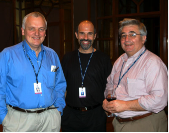
\includegraphics{2.3.png}
\caption{\emph{John Rendon (derecha) en el Foro Highlands, acompañado
por el presentador de la BBC Nik Gowing (izquierda) y Jeff Jonas,
ingeniero en jefe de Entity Analytics de IBM (centro)}}
\end{figure}

TRG es una famosa empresa de comunicaciones que ha sido contratista del
gobierno por décadas. Rendon jugó un papel clave en la implementación de
las campañas de propaganda del departamento de estado en Irak y Kosovo
con Clinton y Metzl. Esto incluyó el recibir una concesión del Pentágono
para mantener un sitio web de noticias, Intercambio de Información de
los Balcanes, y un contrato de la Agencia Estadounidense para el
Desarrollo Internacional (USAID) para promover las ``privatizaciones''.

El papel central de Rendon en ayuda de la administración Bush
publicitando la inexistente amenaza de las armas de destrucción masiva
para justificar una invasión militar de Estados Unidos ahora es bien
sabido. De acuerdo a la famosa descripción de James Bamford en su
investigación seminal en la revista Rolling Stone, Rendon desempeñó un
papel importante en nombre de la administración Bush en la
implementación de la ``gestión de la percepción'' para ``crear las
condiciones para el derrocamiento de Hussein del poder'' bajo contratos
de la CIA y del Pentágono por varios millones de dólares.

Entre las actividades de Rendon estuvo la creación, por encargo de la
CIA, del Congreso Nacional Iraquí (INC) de Ahmed Chalabi, un grupo de
exiliados iraquíes encargados de difundir propaganda, incluyendo gran
parte de la inteligencia falsa sobre armas de destrucción masiva. Ese
proceso había comenzado de manera concertada bajo la administración de
George H. W. Bush, prosiguió con bajo perfil durante la presidencia de
Clinton, hasta su escalada después del 11-S en el mandato de George W.
Bush. Rendon así jugó un papel muy importante en la fabricación de
noticias falsas e inexactas relacionadas con Irak bajo lucrativos
contratos de la CIA y del Pentágono --- y lo hizo en el período
transcurrido hasta la invasión de 2003 como asesor del Consejo de
Seguridad Nacional de Bush: el mismo, por supuesto, que planeó las
invasiones de Afganistán e Irak, logradas con el aporte de los
ejecutivos de Enron que estaban entablando conversaciones
simultáneamente con el Foro Highlands del Pentágono.

Pero eso es la punta del iceberg. Documentos desclasificados muestran
que el Foro Highlands estaba íntimamente involucrado en los procesos
encubiertos por el cual funcionarios clave marcaron el camino a la
guerra en Irak, basados en la guerra de la información.

Un Informe redactado en 2007 por el Inspector General del Departamento
de Defensa revela que uno de los contratistas usados extensivamente por
el Foro Highlands del Pentágono durante y después de la guerra de Irak
no era otro que el grupo Rendon (TRG). TRG fue contratado por el
Pentágono para organizar las sesiones del foro, determinar los temas de
discusión, así como convocar y coordinar sus reuniones. La investigación
del Inspector General había sido motivada por las acusaciones planteadas
en el Congreso sobre el papel de Rendon en la manipulación de la
información para justificar la invasión de 2003 y la ocupación de Irak.
Según el informe del Inspector General:

\begin{quote}
\emph{``\ldots{} el secretario adjunto de defensa para la integración de
las redes e información con la dirección de información usó al grupo
Rendon para llevar a cabo foros que atrajeran a un grupo
interdisciplinario de líderes a nivel nacional. Los foros se componían
de pequeños grupos que discutían información y tecnologías y sus efectos
sobre la ciencia, los procesos organizacionales y de negocios,
relaciones internacionales, economía y seguridad nacional. El grupo
Rendon también llevó a cabo un programa de investigación y entrevistas
para formular y desarrollar temas para el grupo enfocadas al Foro
Highlands. La oficina de la secretaria adjunta de defensa para redes e
integración de información debían aprobar los temas y el grupo Rendon
facilitar las reuniones''.}
\end{quote}

El grupo Rendon, el brazo privado de la propaganda del Pentágono, jugó
así un papel central en dirigir literalmente el proceso del Foro
Highlands del Pentágono que reunió a altos funcionarios del gobierno con
ejecutivos de la industria para generar la estrategia de guerra de la
información del departamento de defensa.

La investigación interna del Pentágono absolvió a Rendon de cualquier
delito. Pero esto no es sorprendente, dado el conflicto de intereses en
juego: el Inspector General en ese momento era Claude M. Kicklighter, un
hombre de Bush, quien había supervisado directamente las principales
operaciones militares de la administración. En 2003, fue director del
equipo de transición de Irak del Pentágono y al año siguiente fue
nombrado asesor especial sobre estabilización y operaciones de seguridad
en Irak y Afganistán para el departamento de estado.

\subsection{El nexo entre la vigilancia y la
propaganda}\label{el-nexo-entre-la-vigilancia-y-la-propaganda}

Aún más, los documentos del Pentágono obtenidos por Bamford en su
historia de Rolling Stone revelaron que Rendon había tenido acceso a
datos de vigilancia ultrasecretos de la NSA para llevar a cabo su labor
en nombre del Pentágono. El grupo Rendon, según indican los documentos
del departamento de defensa, tenía autorización para investigar y
analizar desde información clasificada hasta Top Secret/SCI/SI/TK/G/HCS.

``SCI'' significa información confidencial compartimentada, o sea datos
clasificados con un nivel de seguridad superior a Top Secret, mientras
que ``SI'' significa inteligencia especial, es decir, comunicaciones
altamente secretas interceptadas por la NSA. ``TK'' se refiere a
Talent/Keyhole, nombres en clave para las imágenes obtenidas a partir de
aviones de reconocimiento y satélites espías, mientras que ``G''
significa Gamma, que abarca las intercepciones de comunicaciones de
fuentes extremadamente sensibles y ``HCS'' significa sistema de control
de búsqueda - información de un origen humano muy sensible. En palabras
de Bamford:

\begin{quote}
*" Tomados en conjunto, las siglas indican que Rendon goza de acceso a
la información más secreta de las tres formas posibles de recolección de
inteligencia: espionaje, imágenes satelitales y espías humanos``.*
\end{quote}

En definitiva, el Pentágono había hecho lo siguiente:

\begin{enumerate}
\def\labelenumi{\arabic{enumi}.}
\item
  había contratado a Rendon, una empresa de propaganda;
\item
  le había dado acceso a Rendon a la información más clasificada de la
  comunidad de inteligencia, incluyendo datos de vigilancia de la NSA;
\item
  le había encargado a Rendon que le facilitara al departamento de
  defensa el desarrollo de la estrategia de operaciones de información
  ejecutando el proceso del Foro Highlands;
\item
  y además, otra tarea de Rendon era supervisar la ejecución concreta de
  esta estrategia desarrollada a través del proceso del Foro Highlands,
  en las operaciones de información real de todo el mundo en Irak,
  Afganistán y más allá.
\end{enumerate}

El director ejecutivo del grupo, John Rendon, sigue estrechamente
involucrado en el Foro Highlands del Pentágono, desarrollando
operaciones de información del departamento de defensa en el mundo
musulmán. Su biografía de noviembre de 2014 para el curso ``Líderes
emergentes'' de la Harvard Kennedy School lo describe como ``un
participante en las organizaciones progresistas como el Foro
Highlands'', ``uno de los primeros líderes en emplear el poder de las
tecnologías emergentes en apoyo a la gestión de la información de tiempo
real,'' y un experto en ``el impacto de las nuevas tecnologías de la
información sobre las formas de pensar y comportarse de las
poblaciones''. La biografía de Rendon en Harvard también le atribuye el
diseño y ejecución de ``iniciativas de comunicaciones estratégicas y
programas de información relacionados con las operaciones Amanecer de la
odisea (Libia), Protector unificado (Libia), Guerra global contra el
terrorismo (GWOT), Libertad iraquí, Libertad duradera (Afganistán),
Fuerza aliada y Guardián Conjunto (Kosovo), Escudo del desierto,
Tormenta del desierto (Kuwait), Zorro del desierto (Irak) y Causa Justa
(Panamá), entre otras''.

El trabajo de Rendon en las operaciones de información y gestión de la
percepción también ``ha ayudado a una serie de intervenciones militares
de Estados Unidos'' en otros lugares, así como también a operaciones de
información estadounidenses en Argentina, Colombia, Haití y Zimbabue ---
de hecho, un total de 99 países. Como director político nacional del
partido demócrata y ex director ejecutivo, John Rendon sigue siendo una
figura poderosa en Washington bajo la administración de Obama.

Los registros del Pentágono muestran que el grupo Rendon ha recibido más
de 100 millones de dólares del departamento de defensa desde el año
2000. En 2009, el gobierno de Estados Unidos canceló el contrato sobre
``comunicaciones estratégicas'' con el grupo después de las revelaciones
que se estaba utilizando para discriminar a los periodistas que podrían
escribir historias negativas sobre los militares de EE.UU. en
Afganistán, y promover exclusivamente a los periodistas que apoyaban la
política de Estados Unidos. Sin embargo, en 2010, el gobierno de Obama
contrató nuevamente a Rendon para suministrar servicios de ``engaño
militar'' en Irak.

Desde entonces, el grupo Rendon ha asesorado al Comando de Doctrina y
Entrenamiento del Ejército de Estados Unidos, el comando de operaciones
especiales, y aún está contratado para la oficina del secretario de
defensa, el Comando de Comunicaciones Electrónicas del Ejército de
EE.UU., así como para proporcionar ``apoyo a las comunicaciones'' para
el Pentágono y las embajadas de Estados Unidos en operaciones
antinarcóticos.

El grupo Rendon también cuenta en su página web que ofrece ``Soporte a
la Guerra Irregular'', que incluye ``apoyo operativo y de
planificación'', que ``ayuda a nuestros clientes del gobierno y
militares en el desarrollo de nuevos enfoques para contrarrestar y
erosionar el poder de un adversario, su influencia y su voluntad''. Gran
parte de esta apoyo ha sido en sí perfeccionado durante la última década
o más en el interior del Foro Highlands del Pentágono.

\subsection{Guerra irregular y
seudoterrorismo}\label{guerra-irregular-y-seudoterrorismo}

El vínculo íntimo del Foro Highlands del Pentágono, a través de Rendon,
con las operaciones de propaganda perseguidas por Bush y Obama en apoyo
de la ``guerra prolongada'', demuestra el papel integral de la
vigilancia masiva tanto en la guerra irregular como en las
``comunicaciones estratégicas''.

Uno de los principales partidarios de ambas es el profesor John Arquilla
de la Escuela de Posgrado Naval, el reconocido analista de defensa de
Estados Unidos a quien se le atribuye el desarrollo del concepto de
``guerra en red'', y que hoy defiende abiertamente la necesidad de la
vigilancia masiva y la minería de grandes datos en apoyo de las
operaciones preventivas para frustrar planes terroristas. Se da la
circunstancia de que Arquilla es otro ``miembro fundador'' del Foro
Highlands del Pentágono.

Gran parte de su trabajo sobre las ideas de la ``guerra en red'', la
``disuasión en red'', la ``guerra de la información'' y el ``enjambre'',
producido en gran medida por la RAND bajo contrato del Pentágono, se
incubó en el Foro durante sus primeros años y por lo tanto se convirtió
en parte integral de la estrategia del Pentágono. Por ejemplo, en el
estudio de 1999 de Arquilla sobre RAND, ``El surgimiento de la
Noopolitik: hacia una estrategia de la información estadounidense'', él
y su coautor David Ronfeldt expresan su gratitud a Richard O'Neill ``por
su interés, apoyo y orientación'', y a los ``miembros del Foro
Highlands''por sus comentarios anticipados sobre el estudio. En la mayor
parte de su obra sobre RAND agradece al Foro Highlands y a O'Neill por
su apoyo.

\begin{figure}[htbp]
\centering
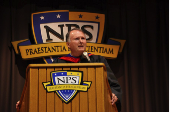
\includegraphics{2.4.png}
\caption{\emph{Prof.~John Arquila de la Escuela de Posgrado Naval,
miembro fundador del Foro Highlands del Pentágono}}
\end{figure}

El trabajo de Arquilla fue citado en una estudio de la Academia Nacional
de Ciencias de 2006 sobre el futuro de la ciencia de la red encargado
por el ejército de Estados Unidos, que encontró, en base ha su
investigación, que ``los avances en las tecnologías basadas en la
informática y las telecomunicaciones están permitiendo a las redes
sociales facilitar las afiliaciones de grupos, incluidas las redes
terroristas''. Además, el estudio fusionó los riesgos de los grupos
terroristas y activistas:``las implicaciones de este hecho para las
redes criminales, terroristas, de protesta y de la insurgencia han sido
exploradas por Arquilla y Ronfeldt (2001) y son un tema común de
discusión de grupos como el Foro Highlands, que perciben que Estados
Unidos es muy vulnerable a la interrupción de las redes críticas''. en
Arquilla pasó a ayudar en el desarrollo de estrategias de guerra de
información ``para las campañas militares en Kosovo, Afganistán e
Irak'', según el historiador militar Benjamin Shearer en su diccionario
biográfico, \emph{Héroes del frente interno} (2007) - que una vez más
ilustra el papel primordial interpretado por algunos miembros clave del
Foro en la ejecución de las operaciones de información del Pentágono en
los teatros de guerra.

En su investigación en \emph{The New Yorker} en 2005, el ganador del
Premio Pulitzer Seymour Hersh se refirió a una serie de artículos de
Arquilla que elaboraron una nueva estrategia de ``lucha contra el
terror'' con pseudo-terror. ``Se necesita una red para combatir una
red'', dijo Arquilla, a partir de la tesis que había estado promoviendo
en el Pentágono a través del Foro Highlands desde su fundación:

\begin{quote}
\emph{``Cuando las operaciones militares convencionales y bombardeos no
lograron derrotar a la insurgencia Mau Mau en Kenia en la década de
1950, los británicos formaron equipos de miembros amigables
pertenecientes a la tribu kikuyu que fingieron ser ser terroristas.
Estas''pseudo-bandas``, como se les llamaba, rápidamente llevaron a los
Mau Mau a la defensiva, ya sea por amistad, para emboscarlos
posteriormente con bandas de combatientes o guiando a los bombarderos a
sus campos militares.''}
\end{quote}

Arquilla se dedicó a abogar para que los servicios de inteligencia
occidentales utilizaran el caso británico como un modelo para la
creación de nuevas ``pseudo bandas'', como grupos terroristas, para
socavar las redes terroristas ``reales'':

\begin{quote}
\emph{``Lo que funcionó en Kenia hace medio siglo tiene una maravillosa
oportunidad de socavar la confianza y el reclutamiento de nuevos
miembros entre las redes terroristas de hoy en día. La formación de
nuevas seudobandas no debería ser difícil.''}
\end{quote}

En esencia, el argumento de Arquilla era que, como sólo las redes pueden
luchar contra las redes, la única manera de derrotar a los enemigos en
una guerra irregular era utilizando técnicas de guerra irregular contra
ellos. En última instancia, el factor determinante en la victoria no es
la derrota militar convencional en sí misma, sino el grado en que la
dirección del conflicto puede ser torcida para influir en la población y
volverla en contra del adversario. La estrategia de ``seudobandas'' de
Arquilla, como informó Hersh, ya ha sido implementada por el Pentágono:

\begin{quote}
\emph{``Bajo el nuevo enfoque de Rumsfeld, me dijeron, agentes militares
estadounidenses podrían hacerse pasar en otros países como empresarios
extranjeros corruptos que buscan comprar artículos de contrabando para
ser utilizados en los sistemas de armas nucleares. En algunos casos,
según los asesores del Pentágono, podrían reclutarse ciudadanos locales
para infiltrarse entre los guerrilleros o terroristas \ldots{}''}
\end{quote}

Las nuevas reglas le permitirán a la comunidad de las fuerzas especiales
establecer lo que llaman ``equipos de acción'' en los países de destino
en el extranjero que pueden utilizarse para encontrar y eliminar las
organizaciones terroristas.``¿Te acuerdas de los escuadrones de
ejecución de derecha en El Salvador?'' me preguntó el ex funcionario de
inteligencia de alto rango, en referencia a las bandas dirigidas por
militares que cometieron atrocidades en los primeros años de la década
del ochenta. ``Nosotros los fundamos y los financiamos'', dijo. ``El
objetivo ahora es reclutar gente en cualquier área que necesitemos. Y no
vamos a decirle al Congreso nada al respecto''. Un ex oficial del
ejército, que tiene conocimiento de las capacidades del comando del
Pentágono, dijo: `vamos a salir a atrapar a los chicos malos'."

La corroboración oficial de que esta estrategia ya está en
funcionamiento se obtuvo a partir de la filtración de un manual de
operaciones especiales de campo del ejército de Estados Unidos del año
2008 . El ejército estadounidense, dice el manual, puede dirigir una
guerra irregular y no convencional mediante el uso de grupos no
estatales sustitutos tales como ``fuerzas paramilitares, particulares,
empresas, organizaciones políticas extranjeras, organizaciones
resistentes o insurgentes, expatriados, adversarios del terrorismo
transnacional, miembros desilusionados del terrorismo transnacional,
comerciantes del mercado negro, y otros''indeseables `sociales o
políticos'``. Sorprendentemente, el manual reconoció expresamente que
las operaciones especiales estadounidenses pueden implicar tanto
contraterrorismo y''terrorismo``, así como''actividades delictivas
transnacionales, incluyendo el narcotráfico, tráfico de armas y las
transacciones financieras ilegales``. El propósito de este tipo de
operaciones encubiertas es, esencialmente, el control de la
población''centrado específicamente en lograr que una parte de la
población local acepte el status quo``, o acepte''cualquier resultado
político" sea éste impuesto o negociado.

Por esta lógica retorcida, el terrorismo puede en algunos casos ser
definido como un instrumento legítimo para que el gobierno
estadounidense influya en la población para que ésta acepte un
``resultado político'' en particular - todo en nombre de la lucha contra
el terrorismo.

¿Es esto lo que el Pentágono estaba haciendo mediante la entrega de
cerca de mil millones de dólares en fondos para los regímenes del Golfo
a los rebeldes anti-Assad, la mayoría de los cuales según las propias
evaluaciones clasificadas de la CIA terminaron en las arcas de los
extremistas islamistas violentos vinculados a Al-Qaeda, que pasaron a
generar el `Estado Islámico'?

El fundamento de la nueva estrategia se estableció oficialmente por
primera vez en una sesión informativa de agosto de 2002 de la Junta de
Ciencias de Defensa del Pentágono, que abogaba por la creación de un
``Grupo de Operaciones Proactivo Preventivo''(P2OG) en el Consejo de
Seguridad Nacional. El P2OG, propuso la junta, debe llevar a cabo
operaciones clandestinas para infiltrarse y ``estimular la reacción'' de
las redes terroristas para provocar que pasen a la acción, y así
facilitar el ataque contra ellas.

La Junta de Ciencias de Defensa, al igual que otras agencias del
Pentágono, está íntimamente relacionada con el Foro Highlands, cuya obra
se alimenta en la investigación de la Junta, que a su vez se presenta
regularmente en el Foro.

Según las fuentes de inteligencia estadounidenses que hablaron con
Hersh, Rumsfeld había asegurado que el nuevo tipo de operaciones oscuras
se llevaría a cabo en su totalidad bajo la jurisdicción del Pentágono,
protegidos por la CIA y los comandantes regionales del ejército
estadounidense, y ejecutado por sus propio comando de operaciones
especiales secretas. Esa cadena de mando incluiría, además del
secretario de Defensa, dos de sus subsecretarios, incluido el
subsecretario de defensa para la inteligencia: la posición supervisada
por el Foro Highlands.

\subsection{Comunicaciones estratégicas: la propaganda de guerra en el
país y en el
extranjero}\label{comunicaciones-estratuxe9gicas-la-propaganda-de-guerra-en-el-pauxeds-y-en-el-extranjero}

Dentro del Foro Highlands, las técnicas de operaciones especiales
exploradas por Arquilla han sido retomadas por muchos otros en
direcciones enfocadas cada vez más en la propaganda - entre ellos, la
Dra. Lochard, como se ha visto anteriormente, y también la Dra. Amy
Zalman, que se centra especialmente en la idea de los militares de
EE.UU. de utilizar ``narrativas estratégicas'' para influir en la
opinión pública y ganar guerras.

Al igual que su colega, el miembro fundador del Foro Highlands Jeff
Cooper, Zalman fue educada en las entrañas de SAIC/Leidos. De 2007 a
2012, ella fue un estratega principal de SAIC, antes de convertirse en
la Dirección de Integración de Información del Departamento de Defensa
en la Escuela Superior de Guerra del Ejército de Estados Unidos, donde
se enfocó en cómo perfeccionar la propaganda para provocar las
respuestas precisas deseadas de los grupos objetivo, basada en la
comprensión completa de esos grupos. Desde el verano del año pasado, se
convirtió en CEO de la Sociedad para el Futuro del Mundo.

\begin{figure}[htbp]
\centering
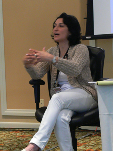
\includegraphics{2.5.png}
\caption{\emph{Dra. Amy Zalman, una ex estratega de SAIC, es CEO de
World Futures Society, y una consultora delegada por el gobierno de los
EE.UU. desde hace mucho tiempo en el Foro Highlands del Pentágono sobre
comunicaciones estratégicas en la guerra irregular.}}
\end{figure}

En 2005, el mismo año en que Hersh informó que la estrategia del
Pentágono de provocar a los terroristas para ``estimular sus
reacciones'' estaba en marcha, Zalman hizo una exposición ante el Foro
Highlands del Pentágono titulada, \emph{En apoyo de un enfoque de la
teoría narrativa para la comunicación estratégica de Estados Unidos}.
Desde entonces, Zalman por largo tiempo delegada del Foro Highlands, y
ha presentado su trabajo en comunicaciones estratégicas a una variedad
de agencias del gobierno estadounidense, foros de la OTAN, así como
cursos de enseñanza sobre guerra irregular a los soldados de la
Universidad de Operaciones Especiales Conjuntas de EE.UU.

Su presentación del Foro Highlands 2005 no está disponible al público,
pero la fuerza del aporte de Zalman en el componente de información de
las estrategias de operaciones especiales del Pentágono se puede deducir
a partir de algunos de sus trabajos publicados. En 2010, cuando aún
formaba parte de SAIC, su artículo de la OTAN señalaba que un componente
clave de la guerra irregular es ``ganar un cierto grado de apoyo
emocional de la población para influir en sus percepciones subjetivas''.
Ella abogó por que la mejor forma de lograr dicha influencia iba mucho
más allá de las técnicas de propaganda y de mensajería tradicionales.
Más bien, los analistas debía ``ponerse en la piel de las personas bajo
observación.''

Zalman lanzó otro artículo el mismo año a través de \emph{IO Journal},
publicado por el Instituto de Operaciones de la Información, que se
describe como un ``grupo de interés especial'' de la Associaton of Old
Crows (AOC) (Nota de Traducción: literalmente, Asociación de Cuervos
Viejos. El nombre de ``Old Crows'' surgió de la primera utilización de
la guerra electrónica en la Segunda Guerra Mundial para interrumpir las
comunicaciones y radares del Eje. Los equipos y operadores aliados eran
conocidos por el nombre de código ``raven'', cuervo. La jerga común
cambió el nombre a ``Crows'' y quienes se dedican a la profesión pasaron
a conocerse como ``Old Crows''. Ambas palabras, raven y crow, se
refieren al cuervo, aunque de diferentes especies. Sin embargo, en
español se usa la misma palabra). La AOC es una asociación profesional
para los teóricos y practicantes de las operaciones de guerra y de
información electrónica, presidida por Kenneth Israel, vicepresidente de
Lockheed Martin, y vicepresidida por David Himes, quien se retiró el año
pasado de su cargo de asesor principal en guerra electrónica en el
Laboratorio de Investigación de la Fuerza Aérea de Estados Unidos.

En este trabajo, titulado \emph{La narración como un factor de
influencia en las Operaciones de Información}, Zalman se lamenta de que
el ejército estadounidense haya ``encontrado dificultades para crear
narrativas convincentes - o historias - ya sea para expresar sus
objetivos estratégicos, o para comunicarse en situaciones delicadas,
tales como las muertes de civiles''. Al final, ella llega a la
conclusión de que ``el complejo tema de las muertes de civiles'' no debe
ser abordado solamente con ``disculpas y compensaciones'' - de todos
modos esto casi ni sucede - sino mediante la propagación de las
narrativas que retratan personajes con los que se conecta la audiencia
(en este caso, ``el público'' son las ``poblaciones en zonas de
guerra''). Esto es para hacer posible que la audiencia decida luchar de
una ``manera positiva'', definida, por supuesto, por los intereses
militares de EE.UU. Involucrarse emocionalmente de esta manera con los
``sobrevivientes de los muertos'' por la acción militar estadounidense
podría ``llegar a ser una forma empática de influencia''. A lo largo de
su trabajo, Zalman es incapaz de cuestionar la legitimidad de los
objetivos estratégicos de Estados Unidos, o reconocer que el impacto de
esos objetivos en la acumulación de las muertes de civiles, es
precisamente el problema que tiene que cambiar - a diferencia de la
forma en que están ideológicamente enmarcadas por las poblaciones
sometidas a la acción militar.

La ``empatía'', en este contexto, es simplemente otro instrumento útil
para manipular.

En 2012, Zalman escribió un artículo para \emph{The Globalist} que
buscaba demostrar cuan necesaria es la delimitación rígida de ``poder
duro'' y ``poder blando'' para superarse, para reconocer que el uso de
la fuerza requiere el efecto simbólico y cultural correcto para
garantizar el éxito:

\begin{quote}
\emph{``Mientras la defensa y la diplomacia económica se encasillen
dentro del''poder duro``, no seremos capaces de ver lo mucho que su
éxito se basa en sus efectos simbólicos, además de los materiales.
Mientras los esfuerzos diplomáticos y culturales se encasillen dentro
del''poder blando``, no seremos capaces de ver las formas en que se
pueden utilizar de manera coercitiva o para producir efectos similares a
los producidos por la violencia''.}
\end{quote}

Dada la profunda participación de SAIC en el Foro Highlands del
Pentágono, y a través de ella el desarrollo de estrategias de
información sobre la vigilancia, la guerra irregular, y la propaganda,
no es de extrañar que SAIC fuera la otra empresa privada clave para
defensa contratada para generar propaganda en el período previo a la
Guerra de Irak de 2003, junto al grupo Rendon.

``Los ejecutivos de SAIC han participado en todas las etapas \ldots{} de
la guerra en Irak'', informó la revista \emph{Vanity Fair},
irónicamente, en términos de la difusión de afirmaciones deliberadamente
falsas sobre armas de destrucción masiva, y luego investigando las
``fallas de inteligencia'' en torno a estas afirmaciones. David Kay, por
ejemplo, que había sido contratado por la CIA en 2003 para buscar armas
de destrucción masiva de Saddam como jefe del Grupo de Investigación en
Irak, hasta octubre de 2002 había sido un vicepresidente principal de
SAIC bajo contrato del Pentágono que machacaba con ``la amenaza
planteada por Irak''. Cuando las armas de destrucción masiva no fueron
halladas, la comisión del presidente Bush para investigar esta ``falla
de inteligencia'' de Estados Unidos incluyó a tres ejecutivos de SAIC,
entre ellos el miembro fundador del Foro Highlands Jeffrey Cooper. El
mismo año del nombramiento de Kay para el Grupo de Investigación en
Irak, el secretario de Defensa de Clinton William Perry - el hombre bajo
cuyas órdenes el Foro Highlands Foro fue puesto en marcha - se unió a la
junta directiva de SAIC. La investigación de Cooper y compañía le
permitió a la administración Bush salirse con la suya con respecto a la
producción de propaganda para legitimar la guerra - como era de
esperarse, dado el papel fundamental de Cooper en la misma red del
Pentágono que fabricaba esa propaganda.

SAIC también fue uno de los muchos contratistas que se beneficiaron
ampliamente con los contratos de reconstrucción de Irak, y fue
contratado nuevamente después de la guerra para promover narraciones
pro-estadounidenses en el extranjero. En la misma línea que la obra de
Rendon, la idea era que las historias plantadas en el extranjero serían
recogidas por los medios de comunicación de Estados Unidos para el
consumo interno.

\begin{figure}[htbp]
\centering
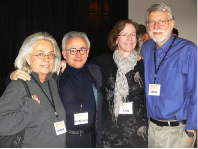
\includegraphics{2.6.png}
\caption{\emph{Delegados del cuadragésimo sexto Foro Highlands del
Pentágono en diciembre de 2011, de derecha a izquierda: John Seely
Brown, jefe científico/director de PARC de Xerox desde 1990 a 2002 y un
antiguo miembro de la junta de In-Q-Tel; Ann Pendleton-Jullian, coautora
junto a Brown del manuscrito, Diseño no consolidado; Antonio y Hanna
Damasio, neurólogo y neurobióloga respectivamente que son parte del
proyecto financiado por DARPA sobre propaganda.}}
\end{figure}

Pero la promoción por parte del Foro Highlands del Pentágono de las
técnicas de propaganda avanzada no es llevada a cabo exclusivamente por
su núcleo, los delegados de larga data como Rendon y Zalman. En 2011, el
Foro hospedó a dos científicos fundadores de DARPA, Antonio y Hanna
Damasio, que son los principales investigadores en el proyecto
\emph{Neurobiología del marco narrativo} de la Universidad de California
del Sur. Evocando el énfasis puesto por Zalman sobre la necesidad de las
operaciones psicológicas del Pentágono para desplegar la ``influencia
empática'', el nuevo proyecto apoyado por DARPA tiene como objetivo
investigar cómo las narrativas suelen apelar ``a los valores sólidos y
sagrados con el fin de provocar una respuesta emocional'', pero de
diferentes formas a través de diferentes culturas. El elemento más
preocupante de la investigación es que se centra en tratar de entender
cómo aumentar la capacidad del Pentágono para desplegar narrativas que
influyan en los oyentes de una manera que invalide el razonamiento
convencional en el contexto de las acciones moralmente cuestionables.

La descripción del proyecto, explica que la reacción psicológica a los
acontecimientos narrados es ``influenciada por cómo enmarca el narrador
los acontecimientos, apelando a diferentes valores, conocimientos y
experiencias del oyente''. El marco de la narrativa que ``se dirige a
los valores sagrados del oyente, incluyendo sus más profundos valores
personales, nacionalistas y/o religiosos, es particularmente eficaz para
influir en la interpretación del oyente de los eventos narrados'',
porque esos ``valores sagrados'' están estrechamente vinculados con ``la
psicología de la identidad, la emoción, la toma de decisiones morales, y
la cognición social''. Mediante la aplicación del encuadre sagrado
incluso en cuestiones mundanas, estas cuestiones ``pueden adquirir
características sagradas y dar lugar a una fuerte aversión a usar el
razonamiento convencional para interpretarlas.'' Los dos Damasios y su
equipo están explorando qué papel desempeñan los ``mecanismos
neuropsicológicos y lingüísticos'' en la determinación de ``la eficacia
del encuadre narrativo utilizando valores sagrados para influir en la
interpretación de los eventos de los oyentes.''

La investigación se basa en la extracción de narrativas de millones de
weblogs estadounidenses, iraníes y chinos, y someterlos a análisis
automatizados del discurso para compararlos cuantitativamente en los
tres idiomas. Los investigadores luego siguieron usando experimentos de
comportamiento con los lectores/oyentes de diferentes culturas para
medir sus reacciones ante las diferentes narrativas" donde cada historia
apela a un valor sagrado para explicar o justificar un comportamiento
moralmente cuestionable del autor``. Por último, los científicos aplican
la exploración neurobiológico fMRI para correlacionar las reacciones y
las características personales de los sujetos con sus respuestas
cerebrales.

¿Por qué la investigación financiada por el Pentágono busca cómo
explotar los ``valores sagrados'' de la gente para extinguir su
capacidad de razonamiento lógico, y aumentar su apertura emocional al
``comportamiento moralmente cuestionable''?

El enfoque en inglés, farsi y chino también puede revelar que las
actuales preocupaciones del Pentágono se refieren casi exclusivamente al
desarrollo de las operaciones de información contra dos adversarios
principales, Irán y China, que encajan perfectamente dentro de las
ambiciones de proyectar influencia estratégica en el Medio Oriente, Asia
Central y el sudeste asiático. De igual modo, el énfasis en el lenguaje
Inglés, específicamente de weblogs estadounidenses, sugiere, además, que
el Pentágono está preocupado por la proyección de la propaganda para
influir en la opinión pública estadounidense.

\begin{figure}[htbp]
\centering
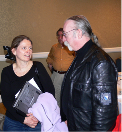
\includegraphics{2.7.png}
\caption{\emph{Rosemary Wenchel (izquierda) del Departmento de Seguridad
Nacional de los EE.UU. junto a Jeff `Skunk' Baxter, un ex músico y ahora
consultor de defensa de EE.UU. que ha trabajado con contratistas como
SAIC y Northrup Grumman. El ejecutivo de SAIC/Leidos, Jeff Cooper,
aparece detrás de ellos.}}
\end{figure}

Para que nadie sospeche que el deseo de DARPA de minar millones de
weblogs estadounidenses como parte de su investigación de la
``neurobiología del encuadre narrativo'' es un simple caso de selección
aleatoria: un copresidente adicional del Foro Highlands del Pentágono en
los últimos años es Rosemary Wenchel, ex directora de capacidades
cibernéticas y operaciones de apoyo a la oficina del secretario de
defensa. Desde 2012, Wenchel ha sido subsecretaria adjunto para la
estrategia y la política del Departamento de Seguridad Nacional.

Como lo demuestra la amplia financiación del Pentágono de la propaganda
en Irak y Afganistán, la influencia de la población y la propaganda es
fundamental no sólo en los teatros remotos del extranjero en regiones
estratégicas, sino también en casa, para sofocar el riesgo de que la
opinión pública nacional socave la legitimidad de la política del
Pentágono. En la foto de arriba, Wenchel está hablando con Jeff Baxter,
un experimentado consultor estadounidense de defensa e inteligencia. En
septiembre de 2005, Baxter fue parte de un grupo de estudio
supuestamente ``independiente'' (presidido por el contratista de la NSA
Booz Allen Hamilton) encargado por el Departamento de Seguridad
Nacional, que recomendó una mayor participación de los satélites espías
estadounidenses en la vigilancia de la población nacional.

Mientras tanto, Zalman y Rendon, que siguen estrechamente involucrados
con el Foro Highlands del Pentágono, continúan siendo cortejados por los
militares de Estados Unidos por su experiencia en las operaciones de
información. En octubre de 2014, ambos participaron en una importante
conferencia de evaluación estratégica multinivel patrocinada por el
Departamento de Defensa de Estados Unidos y el Estado Mayor Conjunto,
titulada \emph{¿Un nuevo paradigma de la Información? Desde los genes
hasta los ``big data'' y desde Instagram hasta la vigilancia persistente
\ldots{} implicaciones para la seguridad nacional}. Otros delegados eran
funcionarios estadounidenses militares de alto rango, ejecutivos de la
industria de defensa, funcionarios de la comunidad de
inteligencia,centro de estudios privados de Washington y académicos.

\begin{figure}[htbp]
\centering
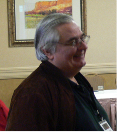
\includegraphics{2.8.png}
\caption{\emph{John Rendon, CEO del Grupo Rendon, en una sesión del Foro
Highlands en 2010.}}
\end{figure}

Rendon y SAIC/Leidos, dos empresas que han sido fundamentales en la
evolución propia de la estrategia de las operaciones de información del
Pentágono a través de su participación fundamental en el Foro Highlands,
continúan siendo contratadas para operaciones clave bajo el gobierno de
Obama. Un documento de la Administración de Servicios Generales del
gobierno estadounidense, por ejemplo, muestra que a Rendon se le
concedió un importante contrato en el período 2010-2015 para
proporcionar servicios de soporte general para las comunicaciones y sus
medios través de las agencias federales. Del mismo modo, SAIC/Leidos
obtuvo un contrato de 400 millones de dólares durante 2010-2015 con el
Laboratorio de Investigación del Ejército de Estados Unidos para
``operaciones de reconstrucción y estabilización en la guerra
expedicionaria, la guerra irregular y las operaciones especiales'' - un
contrato que ``se está preparando ahora para completarlo''.

\subsection{El imperio contraataca}\label{el-imperio-contraataca}

En la administración Obama, el nexo de las empresas, la industria y el
poder financiero representado por los intereses que participan en el
Foro Highlands del Pentágono se ha consolidado en un grado sin
precedentes.

Casualmente, el mismo día en que Obama anunció la renuncia de Hagel, el
Departamento de Defensa emitió un comunicado de prensa destacando cómo
Robert O. Work, subsecretario de defensa de Hagel nombrado por Obama en
2013, planeaba llevar adelante la iniciativa ``Innovación en Defensa''
que Hagel acababa de anunciar una semana antes. La nueva iniciativa se
centraba en garantizar que el Pentágono sufriría una transformación a
largo plazo para mantenerse al día con las principales tecnologías de
punta a través de las operaciones de información.

Cualesquiera que hayan sido las verdaderas razones de la expulsión de
Hagel, esta fue una victoria simbólica y tangible para Marshall y la
visión del Foro Highlands. El copresidente del foro Andrew Marshall,
director de la ONA, puede ciertamente jubilarse. Pero el personal del
Pentágono post-Hagel estará bien provisto con sus seguidores.

Robert Work, que ahora preside el nuevo esquema de transformación del
Departamento de Defensa, es un acólito leal a Marshall que había
dirigido previamente y analizado los juegos de guerra para la oficina de
evaluación de la red. Al igual que Marshall, Wells, O'Neill y otros
miembros del Foro Highlands, Work también es un devoto de los robots,
autor principal del estudio \emph{La preparación para la guerra en la
edad robótica}, publicado en los primeros meses del año anterior por el
``Centro para la Nueva Seguridad Estadounidense'' (CNAS).

Work está decidido a decidir el futuro de la ONA, asistido por su
estratega Tom Ehrhard y por el subsecretario para inteligencia del
Departamento de Defensa, Michael G. Vickers, bajo cuya autoridad el Foro
Highlands funciona actualmente. Ehrard, un defensor de la ``integración
de las tecnologías de punta en el Departamento de Defensa'',
anteriormente se desempeñó como asistente militar de Marshall en la ONA,
mientras que Mike Vickers - que supervisa las agencias de vigilancia
como la NSA - también fue contratado previamente por Marshall como
consultor para el Pentágono.

Vickers es también uno de los principales defensores de la guerra
irregular. Como asistente para operaciones especiales y conflictos de
baja intensidad del ex secretario de Defensa, Robert Gates, tanto en las
administración de Bush como en la de Obama, la visión de la guerra
irregular de Vickers presionó para realizar ``operaciones distribuidas
en todo el mundo'', incluso ``en decenas de países con los que los
EE.UU. no están en guerra'', como parte de un programa de ``guerra
contra la red'' usando una ``red para combatir una red'' - una
estrategia que por supuesto adopta el Foro Highlands por todas partes.
En su puesto anterior bajo el mando de Gates, Vickers aumentó el
presupuesto para las operaciones especiales, incluyendo las operaciones
psicológicas, transporte furtivo, despliegue de drones Predator y
``usando vigilancia de alta tecnología y reconocimiento para rastrear e
identificar a los terroristas e insurgentes''.

Para reemplazar a Hagel, Obama nominó a Ashton Carter, ex subsecretario
de defensa de 2009 a 2013, de quien, por su experiencia en presupuestos
y adquisiciones, según \emph{The Wall Street Journal} se ``espera que
impulse algunas de las iniciativas defendidas por el actual diputado del
Pentágono, Robert Work, incluyendo un esfuerzo para desarrollar nuevas
estrategias y tecnologías para preservar la ventaja de Estados Unidos en
el campo de batalla''.

En 1999, después de tres años como asistente del secretario de defensa
de Clinton, Carter fue coautor de un estudio junto al ex secretario de
defensa William J. Perry donde abogaba por una nueva forma de ``guerra
por control remoto'' facilitada por ``la tecnología digital y el flujo
constante de información''. Uno de los colegas de Carter en el Pentágono
durante su mandato en ese momento era el copresidente del Foro Highlands
Linton Wells; y fue Perry por supuesto que entonces como secretario de
defensa nombró a Richard O'Neill para constituir al Foro Highlands como
centro de estudios de operaciones de información del Pentágono en 1994.

El jefe supremo del Foro Highlands Perry pasó a formar parte del consejo
de SAIC, antes de convertirse finalmente en presidente de otro
contratista gigante de defensa, Global Technology Partners (GTP). Y
Ashton Carter estaba en el consejo de GTP bajo el mando de Perry, antes
de ser nominado para secretario de Defensa de Obama. Durante el anterior
paso por el Pentágono de Carter con Obama, trabajó en estrecha
colaboración con Work y con el actual subsecretario de defensa Frank
Kendall. Fuentes de la industria de defensa se regocijan de que el nuevo
equipo del Pentágono ``mejorará drásticamente'' las oportunidades de
``impulsar a los grandes proyectos de reforma'' en el Pentágono ``para
alcanzar la línea de meta.''

De hecho, la prioridad de Carter como jefe asignado de defensa es la
identificación y adquisición de nueva ``tecnología de punta'' comercial
para mejorar la estrategia militar estadounidense - en otras palabras,
la ejecución del plan Skynet del ministerio de defensa.

Los orígenes de la nueva iniciativa de innovación del Pentágono por lo
tanto se remontan a las ideas que circularon ampliamente dentro del
Pentágono desde hace décadas, pero que no consiguieron arraigarse
plenamente hasta ahora. Entre 2006 y 2010, el mismo período en que esas
ideas estaban siendo desarrollado por los expertos del Foro Highlands
como Lochard, Zalman y Rendon, entre muchos otros, la oficina de
evaluación de la red proporcionó un mecanismo directo para canalizar
esas ideas en estrategias concretas y en el desarrollo de políticas a
través la revisión cuadrienal de defensa, donde el aporte de Marshall
era el principal responsable de la expansión del mundo ``oscuro'':
``operaciones especiales'', ``guerra electrónica'' y ``operaciones de
información''.

\begin{figure}[htbp]
\centering
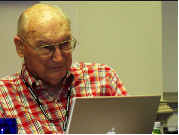
\includegraphics{2.9.png}
\caption{\emph{Andrew Marshall, actualmente jefe retirado de la Oficina
de Evaluación de la Red del Departamento de Defensa de EE.UU. y
codirector del Foro Highlands, en una sesión en 2008.}}
\end{figure}

La visión de Marshall previa al 11-S de un sistema militar totalmente
automatizado y en red se realizó en el estudio Skynet del Pentágono
publicado por la Universidad de Defensa Nacional en septiembre de 2014,
que fue co-escrito por el colega de Marshall en el Foro Highlands,
Linton Wells. Muchas de las recomendaciones de Wells ahora están a punto
de por ser ejecutadas a través de la nueva Iniciativa de Innovación en
Defensa por los veteranos y afiliados de ONA y del Foro Highlands.

Dado que el libro blanco de Wells destacó el gran interés del Pentágono
en acaparar la investigación en inteligencia artificial para monopolizar
la guerra robótica en red autónoma, no es del todo sorprendente que los
socios patrocinadores del Foro de SAIC/Leidos muestren una sensibilidad
extraña sobre el uso público de la palabra ``Skynet''.

En un artículo de Wikipedia titulado \emph{Skynet (fictional)}, las
personas que usan computadoras SAIC borraron varios párrafos en la
sección de curiosidades al señalar ``Skynets'' del mundo real, tales
como el sistema de satélite militar británico, y varios proyectos de
tecnología de información.

La partida de Hagel allanó el camino para que los funcionarios del
Pentágono vinculados al Foro Highlands Foro consolidaran la influencia
del gobierno. Ellos están integrados en una antigua red oculta de
funcionarios políticos, industriales, de los medios de comunicación y de
las corporaciones que se sientan de forma invisible detrás de la sede
del gobierno, y sin embargo, escriben literalmente sus políticas de
seguridad nacional y extranjera, sea la administración demócrata o
republicana, contribuyendo con ``ideas'' y estableciendo relaciones
entre el gobierno y la industria.

Es este tipo de redes a puertas cerradas que ha hecho el inútil voto
estadounidense. Lejos de proteger el interés público o ayudar a combatir
el terrorismo, se ha abusado sistemáticamente del monitoreo exhaustivo
de las comunicaciones electrónicas para potenciar los intereses creados
de las industrias de la energía, la defensa y las tecnologías de la
información.

El estado de guerra global permanente que ha resultado de las alianzas
del Pentágono con contratistas privados y el aprovechamiento sin tener
que rendir cuentas a nadie del amplio conocimiento reunido acerca de la
información, no le brinda seguridad de nadie, sino que ha dado lugar a
una nueva generación de terroristas en forma del llamado ``Estado
islámico'' - un Frankenstein subproducto de la combinación pútrida de la
brutalidad de Assad y las operaciones encubiertas de Estados Unidos
desde hace mucho tiempo en la región. La existencia de este Frankenstein
está siendo cínicamente explotada por los contratistas privados que
buscan beneficiarse de la expansión exponencial del aparato de seguridad
nacional, en momentos en que la volatilidad económica ha presionado a
los gobiernos a recortar el gasto en defensa.

De acuerdo con la Comisión de Bolsa y Valores, de 2008 a 2013, los cinco
mayores contratistas de defensa de Estados Unidos perdieron el 14 por
ciento de sus empleados, con la finalización de las guerras
estadounidenses en Irak y Afganistán como argumento principal de la
escasez de negocios y la reducción de los ingresos. Sus fortunas están
actualmente invertidas en la continuación de la ``guerra prolongada''
desencadenada por ISIS. Las empresas que se benefician de la nueva
guerra incluyen a muchas firmas conectadas al Foro Highlands, como
Leidos, Lockheed Martin, Northrop Grumman y Boeing. La guerra es, de
hecho, un fraude.

\subsection{No más oscuridad}\label{no-muxe1s-oscuridad}

Sin embargo, en el largo plazo, los imperialistas de información ya han
fracasado. Esta investigación se basa enteramente en técnicas de open
source, posibles en gran medida en el contexto de la misma revolución de
la información potenciada por Google. La investigación ha estado
financiada en su totalidad por los miembros del público, a través de
crowdfunding. Y la investigación ha sido publicada y distribuida fuera
de los circuitos de los medios tradicionales, precisamente para plantear
que en esta nueva era digital, las concentraciones verticales y
centralizadas de poder no pueden superar el poder de la gente, su amor a
la verdad y la justicia, y su deseo de compartir.

¿Cuáles son las lecciones de esta ironía? Muy simples, realmente: La
revolución de la información está descentralizada inherentemente, y es
descentralizadora. No puede ser controlada ni cooptada por el Gran
Hermano. Los esfuerzos para hacerlo invariablemente fallarán, de una
manera que será en última instancia contraproducente.

La última iniciativa alocada del Pentágono para dominar el mundo a
través del control de la información mediante la tecnología, no es una
señal de la naturaleza todopoderosa de la red oculta, sino más bien un
síntoma de su crédula desesperación por evitar la aceleración del
declive de su hegemonía.

Pero va por buen camino rumbo a la decadencia. Y esta historia, al igual
que muchas antes que ella, es una pequeña señal de que las oportunidades
para movilizar a la revolución de la información para beneficio de
todos, a pesar de los esfuerzos del poder para ocultarse en las sombras,
están más fuertes que nunca.

\end{document}
